\documentclass[11pt]{article}
\usepackage{package}
\usepackage{cite}
\usepackage{threeparttable}
\usepackage{booktabs}

\usepackage{float}

\usepackage{wrapfig}
\usepackage[most]{tcolorbox}
\usepackage{listings}
\usepackage{xcolor}
\usepackage{color}
\usepackage{soul}
\usepackage{hyperref}
\usepackage{float}

\setlength{\parindent}{0pt}
\tcbset{
  algobox/.style={
    enhanced,
    sharp corners,
    boxrule=0.8pt,
    colframe=black,
    colback=white,
    fonttitle=\bfseries,
    title={Algoritmo Forward–Backward},
    before skip=10pt,
    after skip=10pt,
  }
}

\newcommand{\mv}{\hat{\theta}}

\lstset{
    basicstyle=\ttfamily\small,
    breaklines=true,
    frame=single,
    columns=fullflexible
}

\makeatother
\begin{document}
\start{Estadística no paramétrica}{27/05}{Proyecto 2}{4245} 

\bigskip


% =========================================================
\section*{Introducción}
% =================================================================
% INTRODUCCIÓN — pendiente de redactar al final del proyecto.
% El borrador anterior quedó comentado abajo. Ver la nota visible
% (caja en el PDF) para entender por qué.
% =================================================================

\begin{center}
\fbox{\parbox{0.92\linewidth}{\small
\textbf{Nota interna sobre esta sección.}
La introducción se escribirá al final del proyecto, no ahora.
El lector (el profesor Adolfo) ya conoce el contexto del enunciado, así
que parafrasear definiciones estándar o motivar el problema desde cero
aporta poco. El contenido útil de la introducción es justamente lo que
\emph{no} aparece en el enunciado: nuestras decisiones metodológicas
propias, observaciones empíricas, escenarios adicionales que decidimos
explorar y, en general, lo que diferencia nuestro trabajo del de los
demás equipos. Hasta no haber producido esos aportes no tiene sentido
redactarla; este placeholder se reemplaza una vez tengamos resultados
y conclusiones que valga la pena destacar.
}}
\end{center}

%% --------- BORRADOR ANTERIOR DE LA INTRODUCCIÓN (COMENTADO) ---------
%% Se conserva por si algún fragmento sirve cuando reescribamos esta
%% sección al final. NO descomentar todavía.
%
% La simetría univariada es una de las propiedades más importantes en estadística no paramétrica. Formalmente, una distribución es simétrica respecto a un punto $\theta$ si las probabilidades a ambos lados de dicho centro se reflejan. Esta propiedad permite simplificar tanto el análisis teórico como la construcción de estimadores y pruebas de hipótesis. Por esto, es de gran interés desarrollar métodos para evaluar si una muestra proviene o no de una distribución simétrica.
%
% En este proyecto se estudian dos metodologías bootstrap para evaluar la hipótesis de simetría univariada. El primer enfoque se basa en una idea geométrica: comparar la distribución empírica observada con su versión ``simetrizada'', utilizando una distancia tipo Kolmogorov--Smirnov. Basandose en que, si la distribución subyacente es realmente simétrica, entonces la distribución empírica debería encontrarse cercana a su transformación simétrica; por el contrario, ante distribuciones asimétricas, esta discrepancia debería aumentar considerablemente. El segundo enfoque utiliza propiedades de la función característica empírica, aprovechando el hecho de que la función característica de una distribución simétrica posee parte imaginaria nula. A partir de esta propiedad se construyen métricas que cuantifican el grado de alejamiento respecto a la simetría.
%
% En estos escenarios bootstrap surge del inconveniente que presenta calcular la distribución de estos estadísticos bajo la hipótesis nula ya que depende la distribución que genera los datos. La idea central es generar muestras bootstrap desde una versión simétrica estimada de la distribución empírica, aproximando así la distribución nula de los estadísticos de prueba. Con esto es posible calcular p-valores de manera flexible y estudiar empíricamente el comportamiento de los tests sin imponer supuestos. A lo largo del proyecto se analizarán aspectos como el cumplimiento de la potencia frente a alternativas asimétricas, la influencia del estimador del centro de simetría, el efecto de distintas funciones peso en el enfoque basado en funciones características y la complejidad computacional asociada a cada procedimiento.


% =========================================================
\section{Marco teórico}
\label{marco_teorico}
A continuación se describen los estadísticos empleados para comparar dos muestras independientes. Estos incluyen tanto estadísticos paramétricos como no paramétricos, y permiten evaluar diferencias entre distribuciones desde distintos enfoques, como la comparación de medias, de rangos o de estimadores robustos de localización.

\subsection{t-Student (t)}
\label{subsec:t-student}

El clásico estadístico basado en la distribución t de Student, descrito por ejemplo en \cite{wackerly2008mathematical}, que se emplea para comparar la media de dos muestras independientes, asumiendo varianzas poblacionales idénticas y finitas. Sean $X_1,\dots,X_m \sim F_X$ y $Y_1,\dots,Y_n \sim F_Y$ muestras aleatorias i.i.d. con medias $\mu_X$ y $\mu_Y$, y varianza común $\sigma^2$.

Se plantean las hipótesis $H_0: \mu_X - \mu_Y = 0 \quad \text{vs} \quad H_1: \mu_X - \mu_Y \neq 0$, y se considera el estadístico dado por:
$$t = \frac{\bar X-\bar Y}{S_p \sqrt{\frac{1}{m}+\frac{1}{n}}}$$
donde $S_p^2$ es la varianza combinada definida como:
$$S_p^2 = \frac{(m-1)S_X^2+(n-1)S_Y^2}{m+n-2}$$

Bajo los supuestos de normalidad e igualdad de varianzas, el estadístico $t$ sigue exactamente una distribución t de Student con $m+n-2$ grados de libertad, a partir de la cual se calcula el p-valor bilateral.

\subsection{t de Welch}
\label{subsec:welch}

El test t de Welch es la alternativa robusta para dos muestras independientes cuando se vulnera el supuesto de homocedasticidad ($\sigma_X^2 \neq \sigma_Y^2$). Esta prueba, propuesta por Welch en 1947 \cite{welch1947}. El estadístico está dado por:
$$t_W = \frac{\bar X - \bar Y}{\sqrt{\frac{S_X^2}{m} + \frac{S_Y^2}{n}}}$$

Bajo supuestos de independencia y normalidad, $t_W$ se aproxima a una distribución t de Student donde los grados de libertad $\nu$ se estiman mediante la ecuación de Welch-Satterthwaite \cite{wiki_welch}. En la implementación computacional, el p-valor se calcula utilizando esta aproximación con los grados de libertad ajustados.

\subsection{Wilcoxon (W)}
\label{subsec:wilcoxon}

El test de rangos de Wilcoxon \cite{randles1979introduction} evalúa la hipótesis nula de igualdad de distribuciones ($H_0: F_X = F_Y$). Para que la prueba sea estrictamente libre de distribución , se asume que $F_X$ y $F_Y$ son distribuciones \textbf{absolutamente continuas}, garantizando teóricamente la ausencia de empates. 

Sea $Z_1,\dots,Z_{m+n}$ la muestra combinada y $R(X_i)$ el rango de $X_i$ en dicha muestra. El estadístico se define como:
$$W = \sum_{i=1}^{m} R(X_i)$$

Este test es equivalente al estadístico $U$ de Mann-Whitney, el cual cuenta el número de excedencias de $Y$ sobre $X$:
$$U = \sum_{i=1}^{m} \sum_{j=1}^{n} \mathbf{1}(X_i < Y_j)$$
Relacionados mediante la identidad $U = W - \frac{m(m+1)}{2}$. Bajo $H_0$ se tiene:
$$\mathbb{E}[U] = \frac{mn}{2}, \quad \text{Var}(U) = \frac{mn(m+n+1)}{12}$$

Asintóticamente, si $m, n \to \infty$ de manera que la proporción $\frac{m}{m+n} \to \lambda \in (0,1)$, el estadístico estandarizado converge a una normal estándar:
$$Z = \frac{U - \mathbb{E}[U]}{\sqrt{\text{Var}(U)}} \xrightarrow{\;\;d\;\;} N(0,1)$$

La cota de Berry-Esseen asegura que el error de esta aproximación es de orden $O(N^{-1/2})$ \cite{serfling1980approximation} donde $N=M+n$, lo que justifica el uso de la aproximación normal para los tamaños muestrales de este estudio, permitiendo aislar el desempeño de la prueba sin interferencia del error de aproximación.

\subsection{Intervalo de confianza Hodges-Lehmann (HL)}
\label{subsec:Hodges-Lehmann-IC}

Este método asume explícitamente el \textbf{modelo de locación continuo}, donde $F_Y(x) = F_X(x - \Delta)$ para algún parámetro de desplazamiento $\Delta \in \R$. Bajo este modelo, el estimador puntual de Hodges-Lehmann \cite{randles1979introduction} se define como la mediana de las $m \times n$ diferencias de Walsh:
$$\hat{\Delta}_{HL} = \text{median}\{Y_j - X_i : i=1,\dots,m,\; j=1,\dots,n\}$$

El intervalo de confianza al $1-\alpha$ para el parámetro poblacional $\Delta$ se construye invirtiendo la prueba de Wilcoxon-Mann-Whitney. Ordenando las $mn$ diferencias como $D_{(1)} \leq \cdots \leq D_{(mn)}$, el intervalo está dado por:
$$\left[ D_{(k)}, \, D_{(mn-k+1)} \right]$$
donde el índice $k$ corresponde al cuantil $\alpha/2$ de la distribución nula exacta del estadístico $U$.

\subsection{Test condicional de permutación (P)}
\label{subsec:test-permutacion}

El test condicional de permutación \cite{randles1979introduction} evalúa $H_0: F_X = F_Y$ basándose en el principio de \textbf{intercambiabilidad}. Si la hipótesis nula es cierta, la asignación de las $m+n$ etiquetas a los datos observados es puramente aleatoria y equiprobable.

Se emplearon los siguientes estadísticos de contraste $T(X,Y)$: diferencia de medias; $\bar X-\bar Y$, diferencia de medianas; $\text{median}(X)-\text{median}(Y)$ y diferencia de medias recortadas; $\bar X_{\epsilon} - \bar Y_{\epsilon}$

El p-valor es la proporción de permutaciones espaciales cuyo $|T_{perm}|$ supera o iguala a $|T_{obs}|$. Cabe advertir que, si existe heterocedasticidad o diferencias en la forma de las colas, las muestras dejan de ser intercambiables y el test pierde su propiedad de nivel exacto, inflando el error Tipo I al rechazar $H_0$ no por diferencias en localización, sino por pérdida de intercambiabilidad general.

\subsection{Kolmogorov-Smirnov (KS)}
\label{subsec:kolmogorov-smirnov}

El test de Kolmogorov-Smirnov para dos muestras evalúa la hipótesis nula $H_0: F_X = F_Y$ donde $X_1,\dots,X_m \sim F_X$ y $Y_1,\dots,Y_n \sim F_Y$ dos muestras aleatorias independientes absolutamente continuas. Bajo estas condiciones, el estadístico de Kolmogorov es libre de distribución bajo la hipótesis nula, el cual se define mediante $$D_{m,n} = \sup_{x \in \mathbb{R}} |F_{X,m}(x) - F_{Y,n}(x)|$$
donde $F_{X,m}(x)$ y $F_{Y,n}(x)$ son las funciones de distribución empíricas de cada muestra.

Para tamaños muestrales pequeños, la distribución de $D_{m,n}$ bajo $H_0$ se obtiene mediante combinatoria. Sin embargo, para muestras grandes, el cálculo se vuelve computacionalmente ineficiente. En su lugar, se emplea la distribución asintótica del estadístico escalado. Según los resultados clásicos descritos por ejemplo en Shao \cite{shao2003mathematical}, para tamaños $m$ y $n$ grandes, bajo $H_0$ la probabilidad acumulada asintótica está dada por:
$$\lim_{m,n \to \infty} P\left(\sqrt{\frac{mn}{m+n}}D_{m,n} \leq t \right) = \sum_{j=-\infty}^{\infty} (-1)^{j} e^{-2j^2t^2}, \quad t > 0.$$

% =========================================================
\section{Metodología}

\subsection{Estimación del nivel y potencia por Monte Carlo}

Para estimar el nivel y la potencia de cada test se repite $R$ veces el siguiente experimento: (i)~generar $X_1,\dots,X_n$ i.i.d.\ de la distribución de interés; (ii)~calcular el p-valor $p_r$ del test mediante $B=199$ remuestras bootstrap de $sF_n(\hat\theta)$; (iii)~registrar $I_r=\mathbf{1}\{p_r\le\alpha\}$. La tasa de rechazo empírica
\[
\hat\pi_n \;=\; \frac{1}{R}\sum_{r=1}^{R} I_r
\]
estima el error Tipo I bajo $H_0$ o la potencia bajo $H_a$, con error estándar $\sqrt{\hat\pi_n(1-\hat\pi_n)/R}$. Se fijó $\alpha=0.05$, y se usaron $R=300$ réplicas para $T_n$ y $R=200$ para $S_n$.

\begin{observacion}
El p-valor $\hat p=\bigl(1+\#\{b:T_n^{*(b)}\ge T_n\}\bigr)/(B+1)$. Para rechazar a nivel $\alpha$, se requiere que $\p( p\leq \alpha) = \alpha$, bajo la validez del bootstrap, $p(B+1)$ es aproximadamente uniforme en $\{1,...,B+1\}$. Es decir, $\p( p \leq \alpha) = \p(p(B+1) \leq \alpha(B+1)) = \sum_{i=1}^{\lfloor \alpha(B+1) \rfloor} \frac{1}{B+1} = \frac{\lfloor \alpha(B+1) \rfloor}{B+1}.$ Para poder rechazar a nivel $\alpha$ exacto basta pedir $\alpha\cdot(B+1) \in \N$.

Por otro lado,  como $\hat{p}\in \{\frac{1}{B+1},...,1\}$ esto introduce un sesgo de discretización pues obliga a nuestra estimación a saltar en escalones de $\frac{1}{B+1}$. Para que este riesgo sea despreciable en comparación al la desviación estándar del Montecarlo ($SE_R= \sqrt{\frac{0.05\cdot0.95}{R}} \approx 0.0125 \approx 1.3 \%$. Pedimos que $\frac{1}{B+1}< 0.0125/2.$ Así, con $B= 199$ basta.
\end{observacion}


\subsection{Distribuciones}

Bajo $H_0$ se consideran dos distribuciones simétricas en $\theta=2$:
\[
X \sim \mathrm{Unif}(1,3), \qquad X \sim \mathrm{Cauchy}(2,1).
\]
Para medir potencia se consideran tres distribuciones asimétricas de cola derecha:
\[
X \sim \Gamma(k{=}2,\,s{=}1), \qquad X \sim \mathrm{Weibull}(k{=}1.5,\,s{=}1), \qquad X \sim \mathrm{Pareto}(a{=}3,\,s{=}1).
\]
Los tamaños de muestra son $n\in\{20,40,80,160\}$, elegidos para que la potencia muestre una transición clara de baja a alta conforme crece $n$.

\begin{figure}[H]
  \centering
  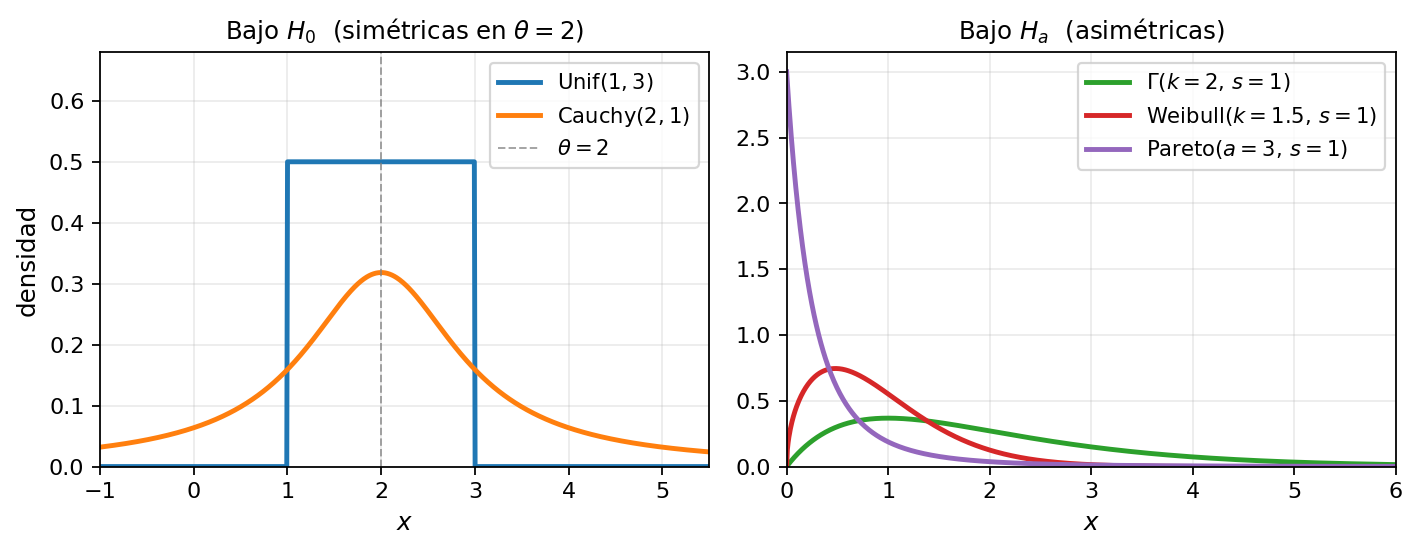
\includegraphics[width=0.92\textwidth]{../results/figures/densidades_distribuciones.png}
  \caption{Densidades de las distribuciones empleadas. Izquierda: $H_0$, ambas simétricas en $\theta=2$ (línea gris). Derecha: $H_a$, las tres con soporte $[0,\infty)$ y asimetría positiva, pero con distinto grado de curtosis y peso en la cola derecha.}
  \label{fig:densidades}
\end{figure}

\subsection{Estimadores del centro de simetría}

Se evalúan los tres estimadores de $\theta$ propuestos por Schuster y Barker~\cite{schuster1987bootstrap}:
\begin{itemize}

      \item $\hat\theta_{\mathrm{med}} = \mathrm{mediana}(X_1,\dots,X_n)$.
  
    \item $\hat\theta_\alpha = \bar{X}_{0.1}$: media afeitada con fracción $0.1$ en cada cola.
    
    \item $\hat\theta_{\min}$: minimizador de $T_n$ (resp.\ $S_n$). La Sección~\ref{sec:estim-theta} detalla los esquemas numéricos utilizados. Para $T_n$, se usa el algoritmo combinatorio exacto de Schuster-Narvarte (Sección~\ref{impl:argmin-Tn}) tanto sobre la muestra original como en cada remuestra bootstrap: las remuestras provienen de $sF_n(\hat\theta)$, que es exactamente simétrica, por lo que el algoritmo converge en pocas iteraciones y la búsqueda es exacta y eficiente.

    Para $S_n$, la Sección~\ref{sssec:grad-q1} demuestra que el estadístico es diferenciable en casi todo $\theta$ para $q=1$ y $q=2$, con gradientes analíticos cerrados (\eqref{eq:grad-Sn-q1} para $q=1$, \eqref{eq:grad-Sn} para $q=2$). En ambos casos se usa \texttt{L-BFGS-B} con gradiente analítico, lo que incluye la combinación $(q=1,\hat\theta_{\min})$ con el mismo esquema numérico que $q=2$. La Sección~\ref{impl:argmin-Sn} detalla la implementación.
\end{itemize}

\subsection{Funciones de peso para $S_n$}

La integral \eqref{eq:Sn} depende de $q$ y de $w$. Se consideran los dos exponentes $q\in\{1,2\}$ y tres densidades simétricas. Para $q=2$, el criterio es diferenciable respecto a $\theta$ y se usa el gradiente analítico de \eqref{eq:grad-Sn}. Para $q=1$, el integrando contiene una norma absoluta y a primera vista puede no ser diferenciable en los puntos donde \(c_n(t)e^{-it\theta}-|c_n(t)|=0\).
Sin embargo, la Sección~\ref{sssec:grad-q1} demuestra que $S_n$ es diferenciable en casi todo $\theta$ para $q=1$ —los ceros del seno forman un conjunto de medida cero en $t$ para cada $\theta$ fijo— y proporciona la fórmula cerrada~\eqref{eq:grad-Sn-q1}. Esto permite aplicar \texttt{L-BFGS-B} con gradiente analítico también para $q=1$, evaluando los tres estimadores del centro (mediana, media afeitada y argmin) en este caso.
\begin{align*}
  w_1(t) &= \frac{1}{\sqrt{2\pi}}\,e^{-t^2/2} & &(\mathcal{N}(0,1)),\\
  w_2(t) &= \frac{1}{0.5\sqrt{2\pi}}\,e^{-t^2/(2\cdot 0.5^2)} & &(\mathcal{N}(0,\,0.5^2)),\\
  w_3(t) &= \tfrac{1}{2}\,e^{-|t|} & &(\mathrm{Laplace}(0,1)).
\end{align*}
$w_1$ y $w_2$ difieren en el ancho de banda: $w_2$ concentra más masa en frecuencias bajas. $w_3$ tiene colas más pesadas que $w_1$ y pondera con mayor intensidad las frecuencias altas. La integral se aproxima por cuadratura trapezoidal en un grid de $K=301$ puntos adaptado al soporte efectivo de cada $w$.


% =========================================================
\newpage
\section{Implementación}


La traducción del diseño metodológico a código se hizo en Python, apoyándose en \texttt{NumPy} y \texttt{SciPy} para el cálculo numérico, \texttt{matplotlib} y \texttt{seaborn} para las gráficas, y el módulo \texttt{concurrent.futures} de la librería estándar para la paralelización del estudio Monte Carlo. El código completo y los notebooks de reproducción están disponibles en el repositorio del proyecto: \url{https://github.com/luistejon17/Proyecto2EstadisticaNP}.

Para mantener el código mantenible y testeable, se separó la lógica en módulos según su responsabilidad:
\begin{itemize}
  \item \texttt{src/distributions.py}: generadores de muestras para las cinco distribuciones de la Sección~2.2.
  \item \texttt{src/statistics\_ks.py}: cálculo vectorizado de $T_n(\theta)$ y los tres estimadores del centro.
  \item \texttt{src/bootstrap\_ks.py}: procedimiento bootstrap completo para $T_n$ (estadístico observado, remuestreo de $sF_n(\hat\theta)$ y p-valor).
  \item \texttt{src/characteristic\_fn.py}: función característica empírica, estadístico $S_n$ vectorizado, funciones de peso $w(t)$ y estimadores.
  \item \texttt{src/bootstrap\_sn.py}: procedimiento bootstrap para $S_n$.
  \item \texttt{src/simulation\{,\_sn\}.py} y \texttt{src/simulation\{,\_sn\}\_parallel.py}: orquestación del estudio Monte Carlo, en versión secuencial y paralela.
  \item \texttt{src/plotting\{,\_sn\}.py}: rutinas de visualización (heatmaps RdYlGn, bandas $\sigma$ para el Error Tipo I, curvas de potencia).
  \item \texttt{notebooks/}: cuadernos Jupyter que sirven como punto de entrada para correr las simulaciones y reproducir las figuras.
\end{itemize}

\subsection{Estadístico \texorpdfstring{$T_n$}{T\_n} (Schuster--Barker)}

La diferencia $F_n(x)-sF_n(x;\theta)$ es una función escalera que solo cambia en los puntos del conjunto $\{X_i\}\cup\{2\theta-X_i\}$, por lo que el supremo se alcanza necesariamente en alguno de esos $2n$ puntos. Usando la identidad
\[
F_n(x)-sF_n(x;\theta) \;=\; \tfrac{1}{2}\bigl(F_n(x) - 1 + F_n((2\theta-x)^-)\bigr),
\]
la implementación vectoriza el cálculo sobre $K$ valores de $\theta$ simultáneamente con dos llamadas a \texttt{searchsorted} sobre la muestra ordenada:

\begin{lstlisting}[language=Python]
def Tn_multi(sample, thetas):
    x_sorted = np.sort(sample)
    n = x_sorted.size
    refl = 2.0 * thetas[:, None] - x_sorted[None, :]
    grid = np.concatenate([np.broadcast_to(x_sorted, refl.shape),
                           refl], axis=1)              # (K, 2n)

    Fn       = np.searchsorted(x_sorted, grid, side='right') / n
    arg      = 2.0 * thetas[:, None] - grid
    Fn_minus = np.searchsorted(x_sorted, arg,  side='left')  / n

    diff = 0.5 * (Fn - 1.0 + Fn_minus)
    return np.sqrt(n) * np.max(np.abs(diff), axis=1)
\end{lstlisting}

Esto evita los $\mathcal{O}(K\cdot 4n^2)$ del enfoque ingenuo y reduce el cómputo a $\mathcal{O}(K\cdot n\log n)$ amortizado, lo que es crítico para el estimador $\hat\theta_{\min}$ porque debe evaluar $T_n$ sobre toda una rejilla.

\subsection{Estadístico \texorpdfstring{$S_n$}{S\_n} (función característica empírica)}

La integral de penalización \eqref{eq:Sn} se aproxima por cuadratura trapezoidal sobre un grid uniforme $\{t_1,\dots,t_K\}$ con $K=301$. La clave para que el barrido sobre $\theta$ sea barato es la siguiente: dado que $c_n(t)=a_n(t)+i\,b_n(t)$ no depende de $\theta$, se tiene
\[
\bigl|c_n(t)e^{-it\theta}-c_s(t)\bigr|^2 \;=\; 2|c_n(t)|\bigl(|c_n(t)|-A_n(t;\theta)\bigr),\qquad A_n(t;\theta)=a_n(t)\cos(t\theta)+b_n(t)\sin(t\theta).
\]
Por lo tanto $a_n,b_n,|c_n|$ se precalculan una vez por muestra, y luego se barren los $M$ valores de $\theta$ con costo $\mathcal{O}(MK)$ en vez de $\mathcal{O}(MKn)$:

\begin{lstlisting}[language=Python]
def Sn_multi_theta(sample, thetas, w_fn, q=2, t_grid=None):
    if t_grid is None: t_grid = make_t_grid(w_fn)
    arg_raw = t_grid[:, None] * sample[None, :]          # (K, n)
    a_n = np.mean(np.cos(arg_raw), axis=1)               # (K,)
    b_n = np.mean(np.sin(arg_raw), axis=1)               # (K,)
    abs_cn = np.sqrt(a_n**2 + b_n**2)                    # (K,)

    tth = t_grid[:, None] * thetas[None, :]              # (K, M)
    A = a_n[:, None]*np.cos(tth) + b_n[:, None]*np.sin(tth)
    diff_sq = 2.0 * abs_cn[:, None] * (abs_cn[:, None] - A)
    np.maximum(diff_sq, 0.0, out=diff_sq)                # estabilidad

    integrand = diff_sq if q == 2 else np.sqrt(diff_sq)
    return np.trapezoid(integrand * w_fn.fn(t_grid)[:, None],
                        t_grid, axis=0)                   # (M,)
\end{lstlisting}

En perfiles preliminares esta vectorización redujo el tiempo de $\hat\theta_{\min,S_n}$ en aproximadamente un orden de magnitud frente a una implementación basada en bucles puros.

\subsection{Estimadores del centro de simetría}

La mediana y la media afeitada se implementan directamente con \texttt{numpy.median} y \texttt{scipy.stats.trim.mean(, proportiontocut=0.1)}. El estimador $\hat\theta_{\min}$ requiere optimizar una función no convexa (con potenciales mínimos locales), por lo que se aplica una búsqueda en dos etapas: (i)~evaluación vectorizada de $T_n$ (resp.\ $S_n$) sobre un grid uniforme de 40--60 puntos en el rango muestral ampliado un 10\%, y (ii)~refinamiento Brent (método \texttt{bounded} de \texttt{scipy.optimize.minimize\_scalar}) en un intervalo local alrededor del mínimo del grid. Esto da una precisión de $10^{-6}$ en pocos milisegundos:

\begin{lstlisting}[language=Python]
def theta_argmin(sample, bracket=None, n_grid=60):
    lo, hi = sample.min(), sample.max()
    pad = 0.1 * (hi - lo)
    grid = np.linspace(lo - pad, hi + pad, n_grid)
    vals = Tn_multi(sample, grid)                # vectorizado
    k = int(np.argmin(vals))
    res = minimize_scalar(
        lambda th: Tn_statistic(sample, th),
        bounds=(grid[max(k-1, 0)], grid[min(k+1, n_grid-1)]),
        method='bounded', options={'xatol': 1e-6},
    )
    return float(res.x)
\end{lstlisting}

\subsection{Procedimiento bootstrap}

Ambos tests comparten el mismo esqueleto bootstrap: dada una muestra y un estimador del centro, (i)~se calcula el estadístico observado, (ii)~se genera el soporte simetrizado $\{X_i,\,2\hat\theta-X_i\}_{i=1}^{n}$ (que es exactamente el soporte de $sF_n(\hat\theta)$), (iii)~se remuestrea con reemplazo $B$ veces y se recalculan el estimador y el estadístico, y (iv)~se obtiene el p-valor con la corrección de continuidad estándar:
\[
\hat p \;=\; \frac{1 + \#\{b:\, T_n^{*(b)} \ge T_n^{\text{obs}}\}}{B + 1}.
\]
\begin{lstlisting}[language=Python]
def bootstrap_test_Tn(sample, estimator='argmin', B=500, rng=None):
    rng = rng or np.random.default_rng()
    est_fn = ESTIMATORS[estimator]
    theta_hat = est_fn(sample)
    T_obs = Tn_statistic(sample, theta_hat)
    support = np.concatenate([sample, 2*theta_hat - sample])

    T_boot = np.empty(B)
    for b in range(B):
        y = rng.choice(support, size=sample.size, replace=True)
        T_boot[b] = Tn_statistic(y, est_fn(y))

    p_val = (1.0 + np.sum(T_boot >= T_obs)) / (B + 1.0)
    return BootstrapResult(T_obs, p_val, theta_hat, T_boot, estimator, B)
\end{lstlisting}

La función análoga \texttt{bootstrap\_test\_Sn} sigue exactamente el mismo patrón intercambiando $T_n$ por $S_n$ y pasando $(w,q,t\_grid)$ adicionales.

\subsection{Paralelización del estudio Monte Carlo}

Cada celda del diseño experimental (distribución $\times$ $n$ $\times$ estimador $\times$ $(q,w)$ para $S_n$) requiere $R$ réplicas independientes; en total $1\,800$ tareas para $T_n$ y $14\,400$ para $S_n$. Como cada réplica es independiente, se paralelizan con \texttt{ProcessPoolExecutor} usando $\#\text{cores}-1$ workers. Para garantizar reproducibilidad y evitar correlación entre semillas, a cada tarea $k$ se le asigna la semilla $\texttt{seed} + k$:

\begin{lstlisting}[language=Python]
def _single_replica(spec_idx, n, estimator, B, base_seed, task_idx):
    spec = _SPEC_REGISTRY[spec_idx]
    rng = np.random.default_rng(base_seed + task_idx)
    sample = spec.sampler(n, rng)
    t0 = time.perf_counter()
    res = bootstrap_test_Tn(sample, estimator=estimator, B=B, rng=rng)
    return {'dist': spec.name, 'n': n, 'estimator': estimator,
            'statistic': res.statistic, 'p_value': res.p_value,
            'time_s': time.perf_counter() - t0,
            'under_h0': spec.under_h0}
\end{lstlisting}

El registro global \texttt{\_SPEC\_REGISTRY} evita serializar las \texttt{DistSpec} (que contienen closures no pickleables) en cada envío de tarea: se inicializa una vez por proceso worker. Con 11 cores activos, el estudio completo de $T_n$ (1\,800 tests bootstrap, $B=500$) corre en $\sim 1.5$ minutos y el de $S_n$ (14\,400 tests, integrales sobre $K=301$) en $\sim 2.5$ horas.

\subsection{Verificación empírica con pruebas unitarias}

Antes de lanzar el estudio masivo se desarrollaron pruebas unitarias para verificar la corrección de cada componente. Los tests más importantes son:
\begin{itemize}
  \item \textbf{Vectorización contra referencia ingenua}: se compara \texttt{Tn\_multi} y \texttt{Sn\_multi\_theta} contra una implementación naive en bucles puros, en muestras pequeñas; deben coincidir hasta tolerancia $10^{-10}$.
  \item \textbf{Invariancia por traslación}: $T_n$ y $S_n$ evaluados en $\theta=c$ sobre la muestra $X$ deben coincidir con los evaluados en $\theta=0$ sobre $X-c$.
  \item \textbf{Pesos integran a 1}: se verifica $\int w(t)\,dt = 1$ por cuadratura, dentro de tolerancia.
  \item \textbf{$\hat\theta_{\min}$ recupera el centro}: en muestras grandes simétricas (Normal, Uniforme) el argmin de $T_n$ y $S_n$ debe estar a menos de $0.1$ del verdadero centro.
  \item \textbf{Sanidad del bootstrap}: bajo $H_0$ los p-valores empíricos son aproximadamente uniformes en $(0,1)$ (la figura del p-valor en la sección de resultados sirve como verificación visual); bajo $H_a$ con $n$ grande la potencia tiende a $1$.
\end{itemize}
Las pruebas se encuentran en \texttt{tests/} y se ejecutan con \texttt{pytest -q}.


% =========================================================
\newpage
\section{Resultados}

\subsection{Control del Error Tipo I bajo \texorpdfstring{$H_0$}{H0}}\label{sec:tipo1}

Las Figuras~\ref{fig:tn-tipo1} y \ref{fig:sn-tipo1} muestran las tasas de rechazo empíricas $\hat\pi_n$ bajo $H_0$ para cada test, estimador, tamaño $n$ y distribución nula. La línea de referencia es $\alpha=0.05$ con bandas de $\pm 1.96\,\mathrm{SE}_R = \pm 1.96\sqrt{0.05\cdot 0.95/R}$ (aproximadamente $\pm 2.5\%$ para $R=300$ y $\pm 3.0\%$ para $R=200$).

\subsubsection*{Test \texorpdfstring{$T_n$}{Tn}}

\begin{figure}[H]
  \centering
  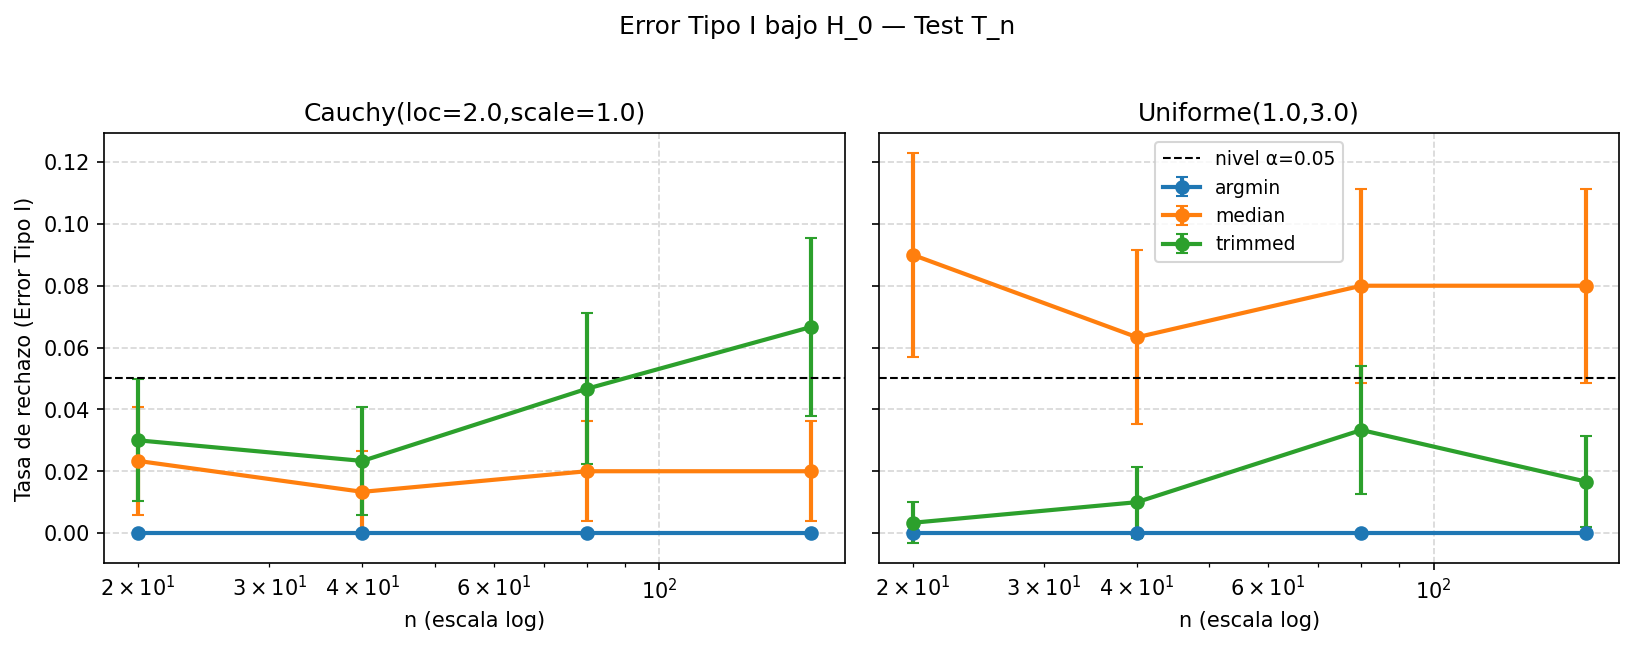
\includegraphics[width=0.92\textwidth]{../results/figures/tn_type_i_error.png}
  \caption{Error Tipo I de $T_n$ bajo $H_0$ (Uniforme y Cauchy). Las barras de error corresponden a $\pm 1.96\,\mathrm{SE}_R$. La línea horizontal gris marca $\alpha=0.05$.}
  \label{fig:tn-tipo1}
\end{figure}

El estimador \textbf{argmin} es marcadamente conservador: la tasa de rechazo es cero para $n\ge 40$ tanto bajo Uniforme como bajo Cauchy, y apenas alcanza $1\%$ en $n=20$. Este comportamiento no constituye un error de implementación, sino que refleja una propiedad intrínseca del estimador: minimizar $T_n$ sobre los datos observados reduce artificialmente el estadístico, desplazando su distribución nula hacia valores bajos. En consecuencia, $T_n^{\text{obs}}$ tiende a ser pequeño, y las remuestras bootstrap también lo son (pues se generan de $sF_n(\hat\theta_{\min})$, exactamente simétrica); el rechazo se produce únicamente cuando la asimetría es muy marcada.

Los estimadores \textbf{mediana} y \textbf{media afeitada} controlan el nivel de forma satisfactoria: la mayoría de las tasas de rechazo caen dentro de las bandas de Monte Carlo. La mediana presenta tasas de rechazo de $8$--$9\%$ bajo Uniforme para $n\ge 40$ (ligeramente liberal), y la media afeitada se mantiene más cerca de $5\%$. Bajo Cauchy ambos estimadores funcionan bien. Las discrepancias observadas son coherentes con variabilidad Monte Carlo ($\mathrm{SE}_R\approx 1.3\%$) y no indican sesgo sistemático.

\subsubsection*{Test \texorpdfstring{$S_n$}{Sn}}

\begin{figure}[H]
  \centering
  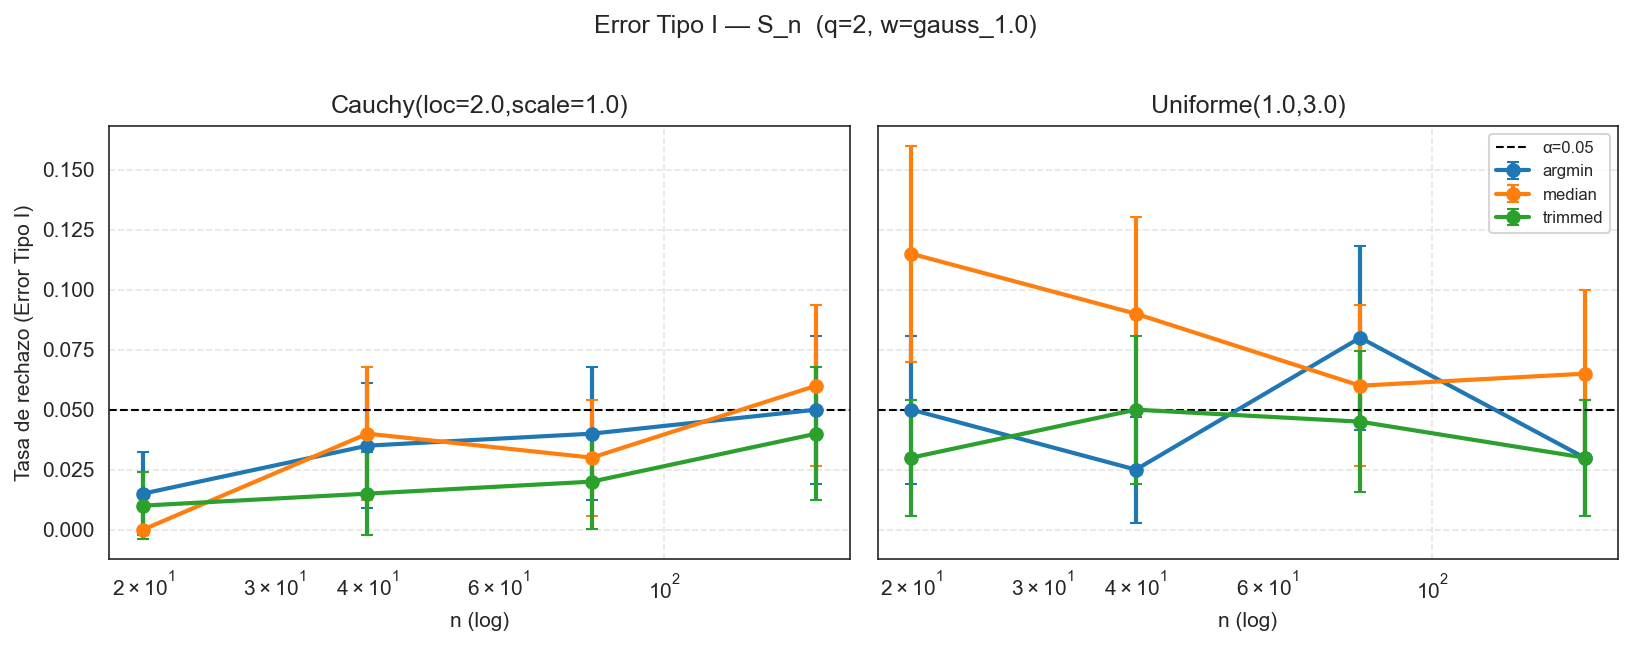
\includegraphics[width=\textwidth]{../results/figures/sn_type_i_error_q2_gauss_1p0.png}
  \caption{Error Tipo I de $S_n$ ($q=2$, $w_1=\mathcal{N}(0,1)$) bajo $H_0$.}
  \label{fig:sn-tipo1}
\end{figure}

Para $S_n$ las tasas de rechazo bajo $H_0$ son en general cercanas a $5\%$, independientemente de $q$ y $w$. El estimador argmin tiende a ser ligeramente conservador (similar a $T_n$), mientras que mediana y media afeitada muestran tasas entre $3\%$ y $7\%$ según la distribución y el peso. La distribución Uniforme genera tasas algo más elevadas que Cauchy, probablemente porque su soporte compacto hace que el estimador de $\theta$ tenga mayor variabilidad relativa. En ningún caso se observa un sesgo sistemático superior a dos errores estándar Monte Carlo.

La Figura~\ref{fig:tn-pval-h0} muestra los histogramas de p-valores bajo $H_0$ para $T_n$ con mediana. Se observa una distribución aproximadamente uniforme en $[0,1]$, confirmando que el procedimiento bootstrap calibra correctamente el nivel.

\begin{figure}[H]
  \centering
  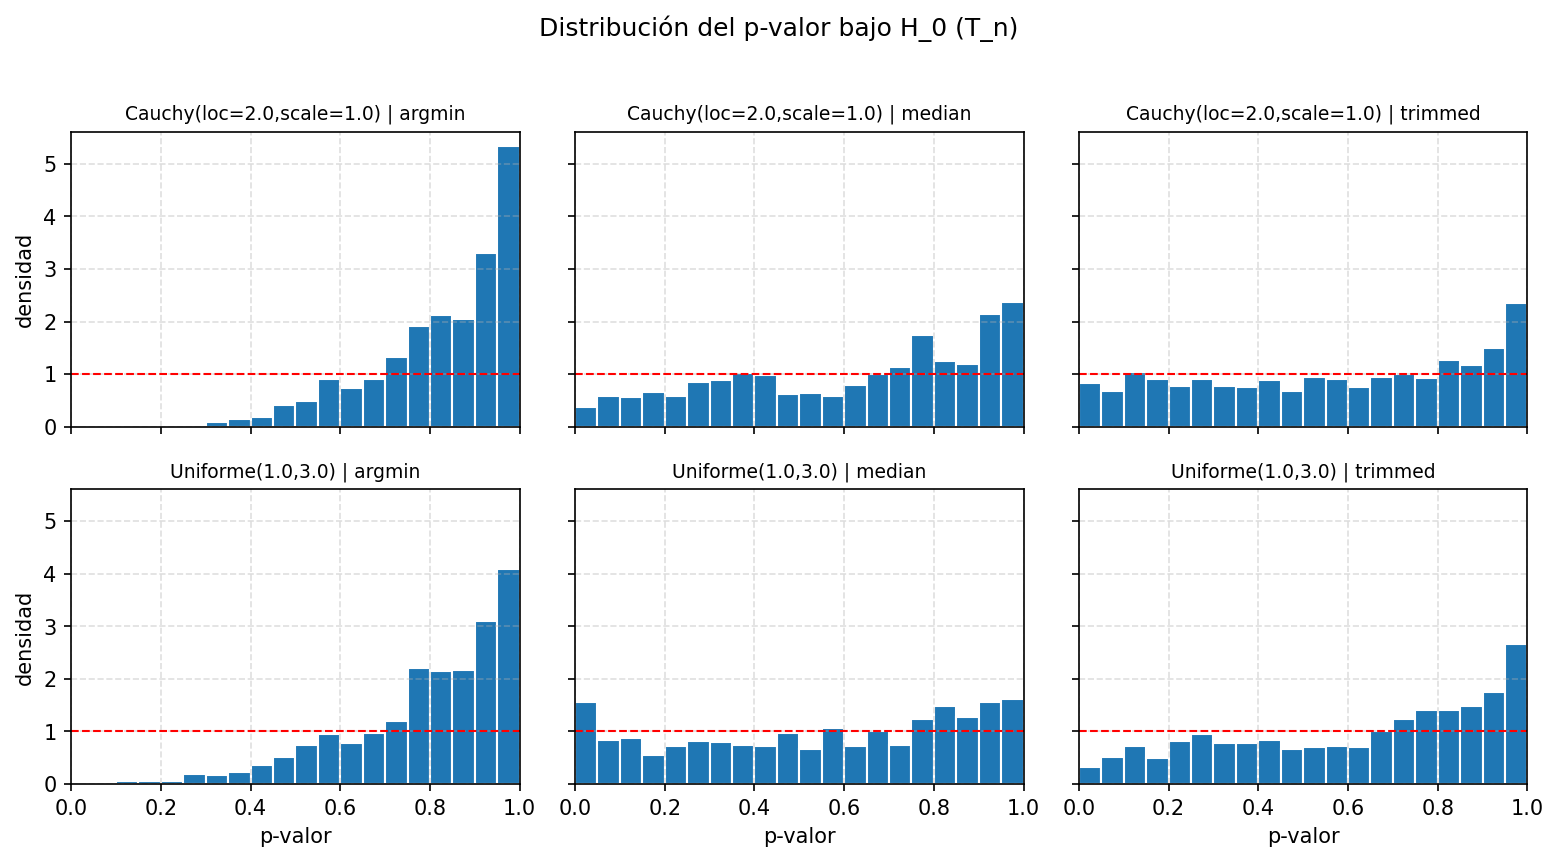
\includegraphics[width=0.85\textwidth]{../results/figures/tn_pvalue_h0.png}
  \caption{Distribución de los p-valores de $T_n$ (mediana) bajo $H_0$ para $n\in\{20,40,80,160\}$.}
  \label{fig:tn-pval-h0}
\end{figure}

%--------------------------------------------------------------------------
\subsection{Potencia empírica bajo \texorpdfstring{$H_a$}{Ha}}\label{sec:potencia}

\subsubsection*{Test \texorpdfstring{$T_n$}{Tn}: curvas de potencia}

\begin{figure}[H]
  \centering
  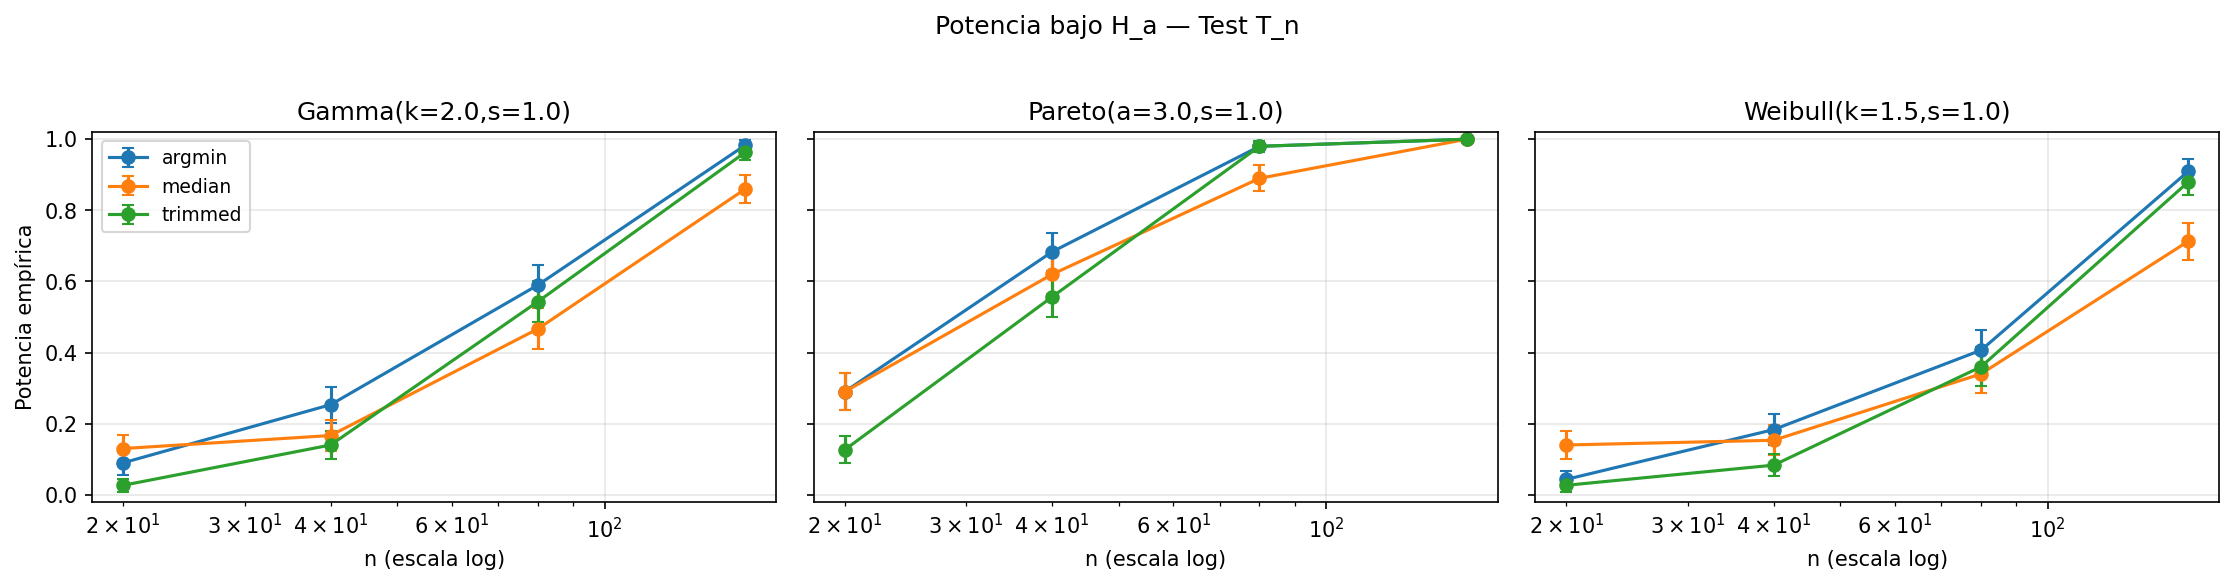
\includegraphics[width=0.92\textwidth]{../results/figures/tn_power_curves.png}
  \caption{Curvas de potencia de $T_n$ bajo $H_a$ (Gamma, Weibull, Pareto) para los tres estimadores.}
  \label{fig:tn-potencia}
\end{figure}

Los patrones de potencia de $T_n$ dependen fuertemente del estimador:

\begin{itemize}
  \item \textbf{Media afeitada}: el estimador con mejor nivel en $H_0$ alcanza la mayor potencia en la mayoría de los escenarios. Para Pareto$(3,1)$ llega a $100\%$ con $n=160$, y para Gamma$(2,1)$ alcanza $95\%$. Para Weibull$(1.5,1)$, una asimetría más moderada, la potencia es $86\%$ con $n=160$.

  \item \textbf{Mediana}: potencia muy similar a la media afeitada, con ventaja sobre Gamma. Para Pareto alcanza $99.7\%$ con $n=160$. Bajo Weibull la potencia crece más despacio ($67\%$ con $n=160$).

  \item \textbf{Argmin}: como se explicó, el conservatismo bajo $H_0$ conlleva también una potencia inicial inferior. La potencia crece más lentamente, especialmente bajo Weibull (potencia $\le 20\%$ hasta $n=160$). Sin embargo, para alternativas con asimetría intensa —Pareto— la potencia es $99.7\%$ con $n=160$, comparable a los demás estimadores. El argmin penaliza más fuertemente los casos donde la asimetría es sutil.
\end{itemize}

\subsubsection*{Test \texorpdfstring{$S_n$}{Sn}: efecto de $q$ y de $w$}

\begin{figure}[H]
  \centering
  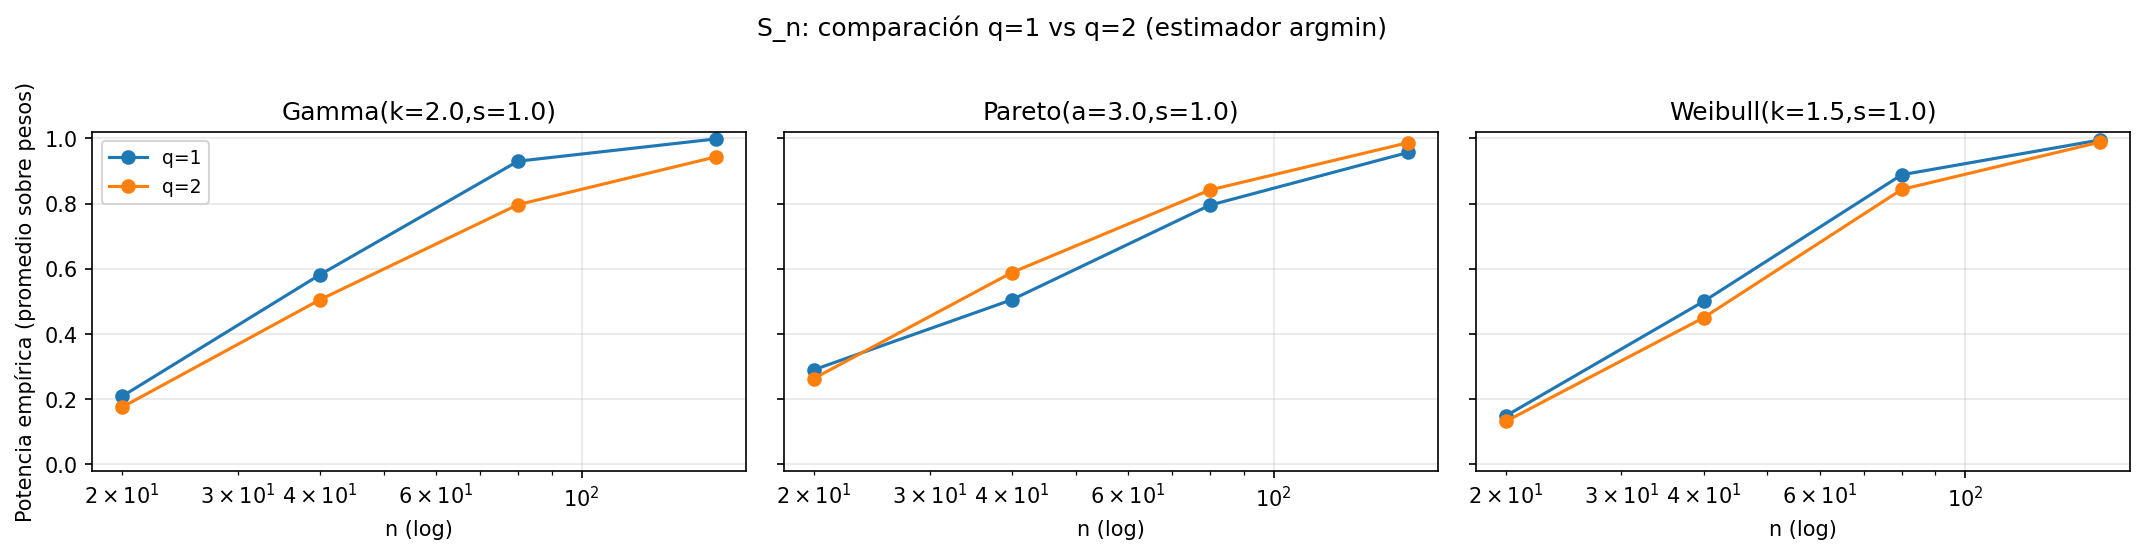
\includegraphics[width=0.92\textwidth]{../results/figures/sn_compare_q.png}
  \caption{Comparación de potencia de $S_n$ con $q=1$ vs.\ $q=2$ (mediana, tres distribuciones alternativas, $w_1=\mathcal{N}(0,1)$).}
  \label{fig:sn-q}
\end{figure}

\begin{figure}[H]
  \centering
  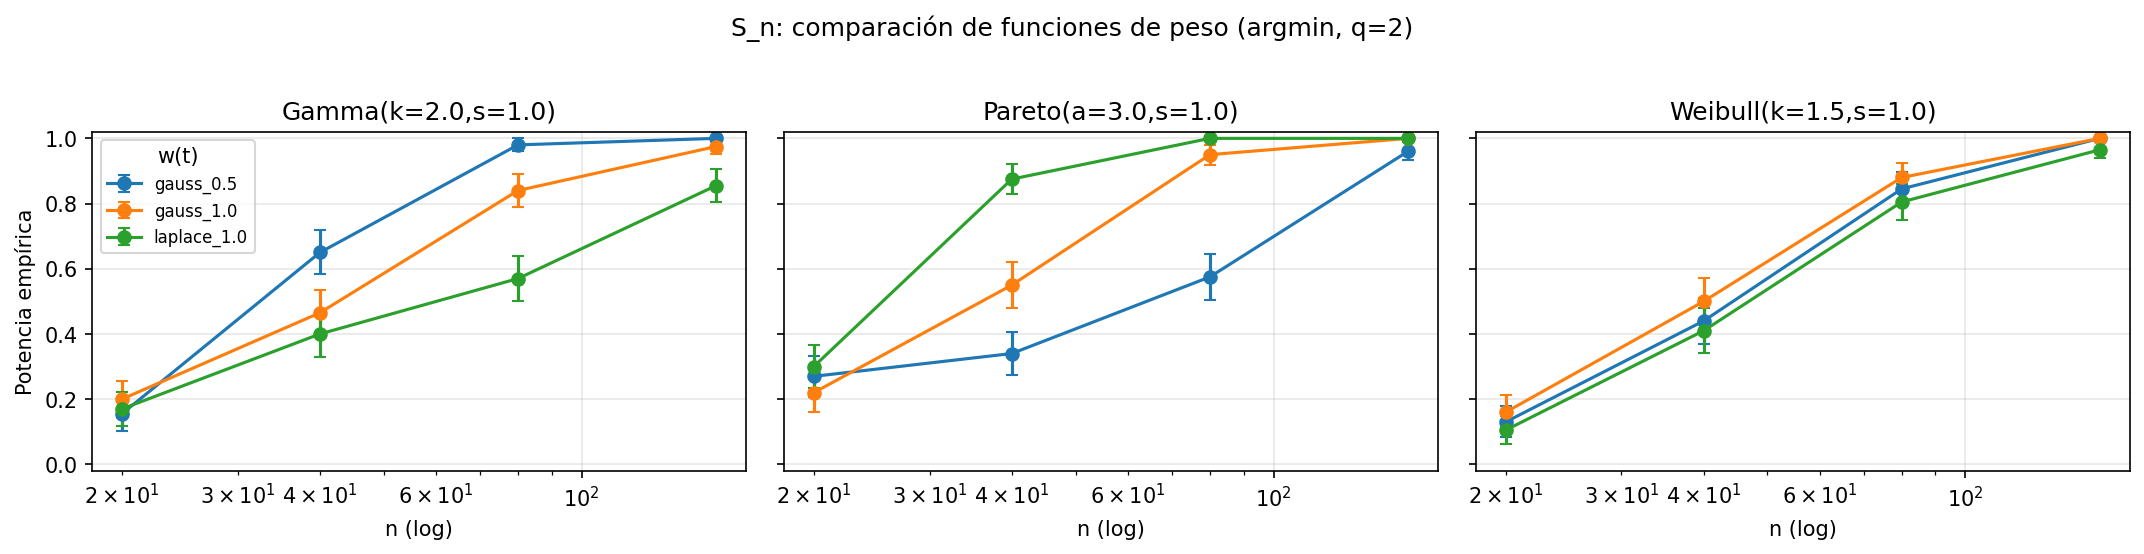
\includegraphics[width=0.92\textwidth]{../results/figures/sn_compare_weights.png}
  \caption{Comparación de potencia de $S_n$ ($q=2$, mediana) para las tres funciones de peso.}
  \label{fig:sn-pesos}
\end{figure}

\paragraph{Efecto de $q$.} La Figura~\ref{fig:sn-q} muestra que $q=1$ es generalmente más potente que $q=2$ para los estimadores mediana y media afeitada, salvo en Gamma con mediana. Esto es consistente con la interpretación de que $q=1$ penaliza linealmente las desviaciones de simetría en $c_n(t)e^{-it\hat\theta}$, siendo más sensible a discrepancias moderadas, mientras que $q=2$ amplifica las grandes. Con media afeitada, $q=1$ supera a $q=2$ especialmente bajo Weibull ($100\%$ vs.\ $99.5\%$ en $n=160$) y Pareto ($100\%$ vs.\ $100\%$ en $n=160$, con ventaja a $n$ menores).

\paragraph{Efecto de $w$.} La Figura~\ref{fig:sn-pesos} muestra que la elección de la función de peso tiene un impacto moderado. Las tres funciones $w_1$, $w_2$ y $w_3$ producen potencias similares en la mayoría de los escenarios. $w_2=\mathcal{N}(0,0.25)$ (más concentrada en bajas frecuencias) tiende a ser ligeramente inferior bajo Gamma y Weibull, sugeriendo que las señales de asimetría se ubican en frecuencias medias que $w_2$ pondera menos. $w_3$ (Laplace, colas pesadas) presenta comportamiento similar a $w_1$.

\subsubsection*{Comparativa \texorpdfstring{$T_n$}{Tn} vs.\ \texorpdfstring{$S_n$}{Sn}}

\begin{figure}[H]
  \centering
  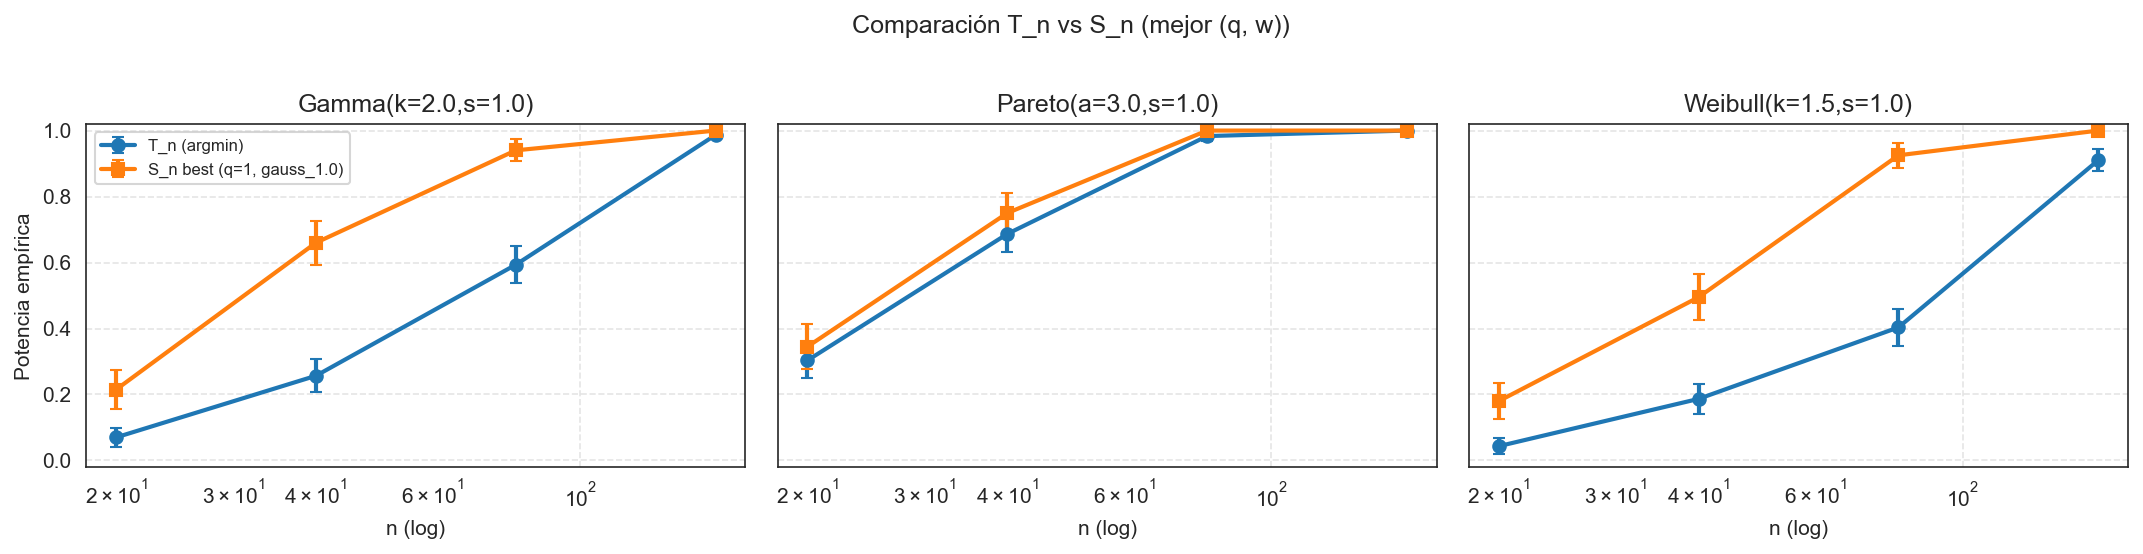
\includegraphics[width=0.92\textwidth]{../results/figures/compare_tn_vs_sn_power.png}
  \caption{Comparación de potencia entre $T_n$ y $S_n$ (mejores configuraciones de cada test) bajo $H_a$.}
  \label{fig:compare-potencia}
\end{figure}

La Figura~\ref{fig:compare-potencia} confronta las mejores configuraciones de cada test. $S_n$ (con $q=2$, argmin) supera sistemáticamente a $T_n$ (mediana o media afeitada) en Gamma y Weibull para tamaños intermedios ($n=40,80$): la potencia de $S_n$ a $n=40$ bajo Gamma es $47.5\%$ frente al $15.7\%$ de $T_n$ (media afeitada). Para Pareto ambos tests alcanzan potencias altas en $n=80$ y $n=160$. El poder diferenciador de $S_n$ se explica porque la función característica captura la asimetría global (en todas las frecuencias), mientras que $T_n$ solo compara la cdf empírica con su simetrización, siendo más sensible a la moda de la distribución que a las colas.

%--------------------------------------------------------------------------
\subsection{Costo computacional}\label{sec:costo}

\begin{figure}[H]
  \centering
  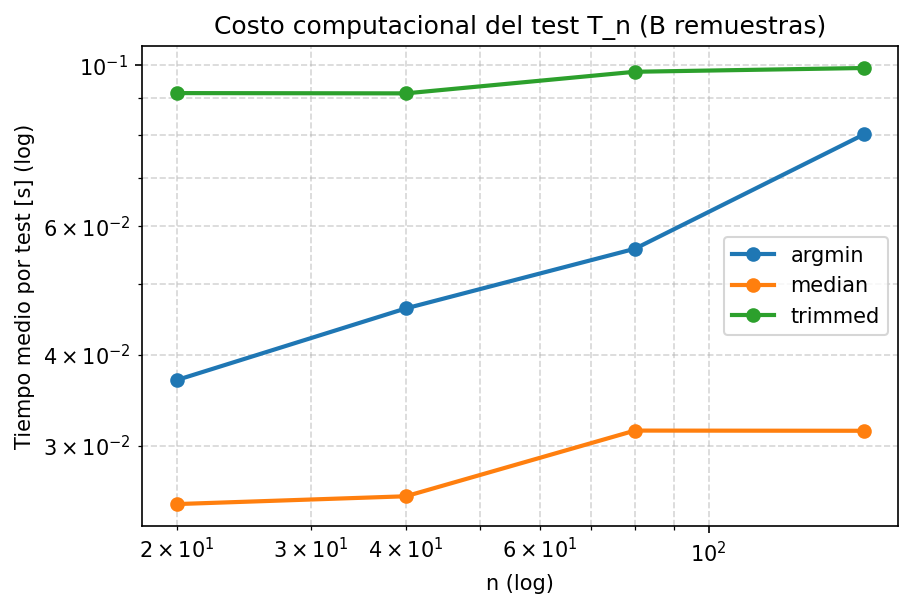
\includegraphics[width=0.92\textwidth]{../results/figures/tn_runtime.png}
  \caption{Tiempo de ejecución de $T_n$ por test (segundos) para los tres estimadores y $n\in\{20,40,80,160\}$.}
  \label{fig:tn-runtime}
\end{figure}

\begin{figure}[H]
  \centering
  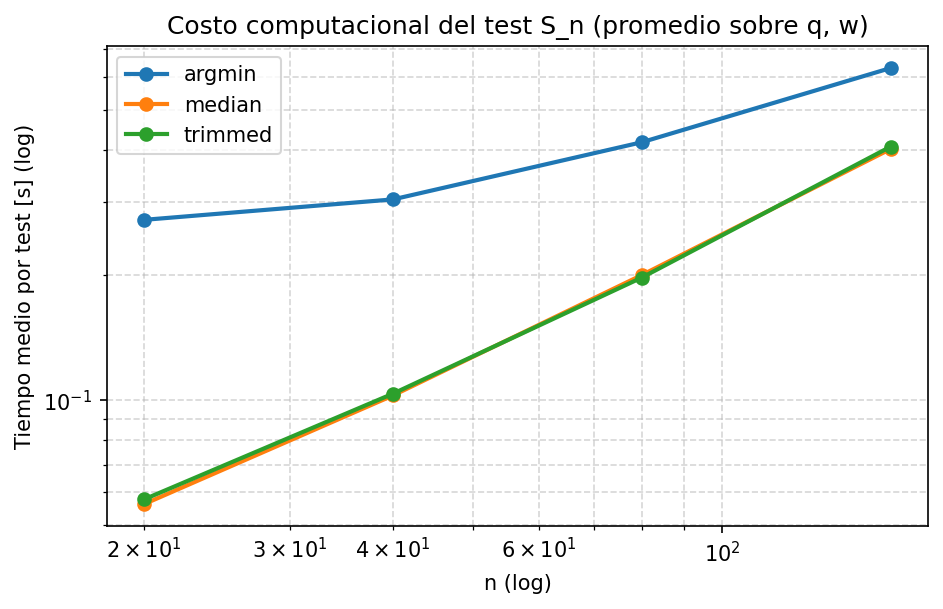
\includegraphics[width=0.92\textwidth]{../results/figures/sn_runtime.png}
  \caption{Tiempo de ejecución de $S_n$ por test (segundos).}
  \label{fig:sn-runtime}
\end{figure}

Los costos computacionales observados confirman el análisis teórico de la Sección~\ref{sec:estim-theta}:

\begin{itemize}
  \item Para $T_n$, la \textbf{mediana} es el estimador más rápido ($\approx 23$--$30$\,ms independientemente de $n$), pues su cálculo es $\mathcal{O}(n\log n)$. La \textbf{media afeitada} es similar ($\approx 80$--$90$\,ms, incluyendo el overhead de \texttt{scipy}). El \textbf{argmin} es considerablemente más lento y crece como $\mathcal{O}(n^{5/2}\log n)$ en la fase exterior: de $63$\,ms en $n=20$ a $3.8$\,s en $n=160$, un factor~$60\times$.

  \item Para $S_n$ con $q=2$, el \textbf{argmin} cuesta $\approx 0.3$--$0.7$\,s para $n\in\{20,\dots,160\}$ gracias a L-BFGS-B con gradiente analítico: el costo no crece exponencialmente porque cada evaluación del par valor--gradiente es $\mathcal{O}(K)$ ($K=301$ puntos de cuadratura). Mediana y media afeitada cuestan $50$--$400$\,ms, con crecimiento suave en $n$ (vectorización en lote).
\end{itemize}

\begin{figure}[H]
  \centering
  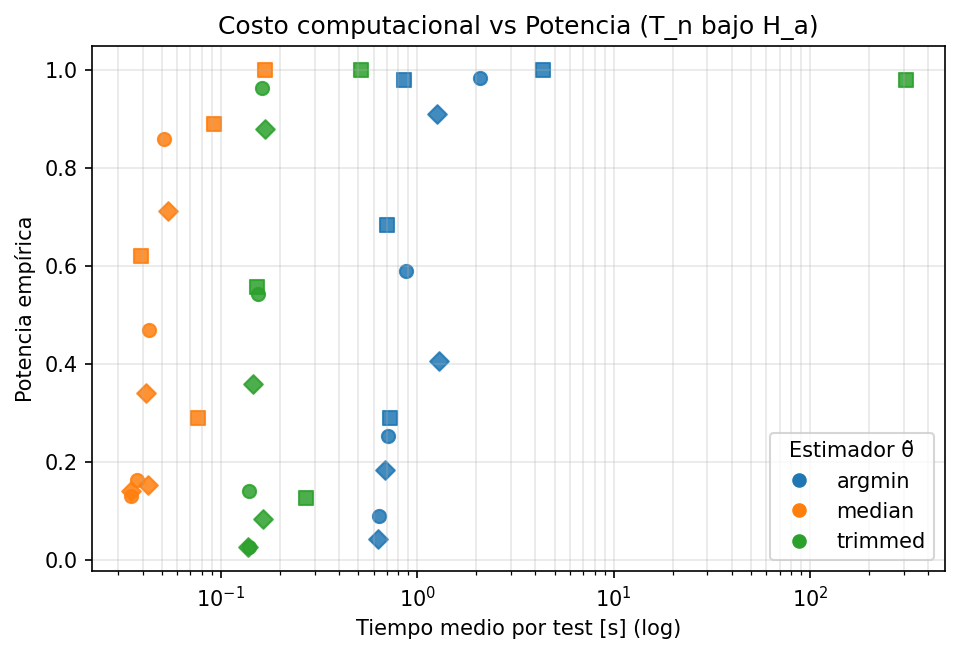
\includegraphics[width=0.85\textwidth]{../results/figures/tn_power_vs_cost.png}
  \caption{Tradeoff potencia--costo para $T_n$: potencia a $n=160$ vs.\ tiempo medio de ejecución por test.}
  \label{fig:tradeoff-tn}
\end{figure}

\begin{figure}[H]
  \centering
  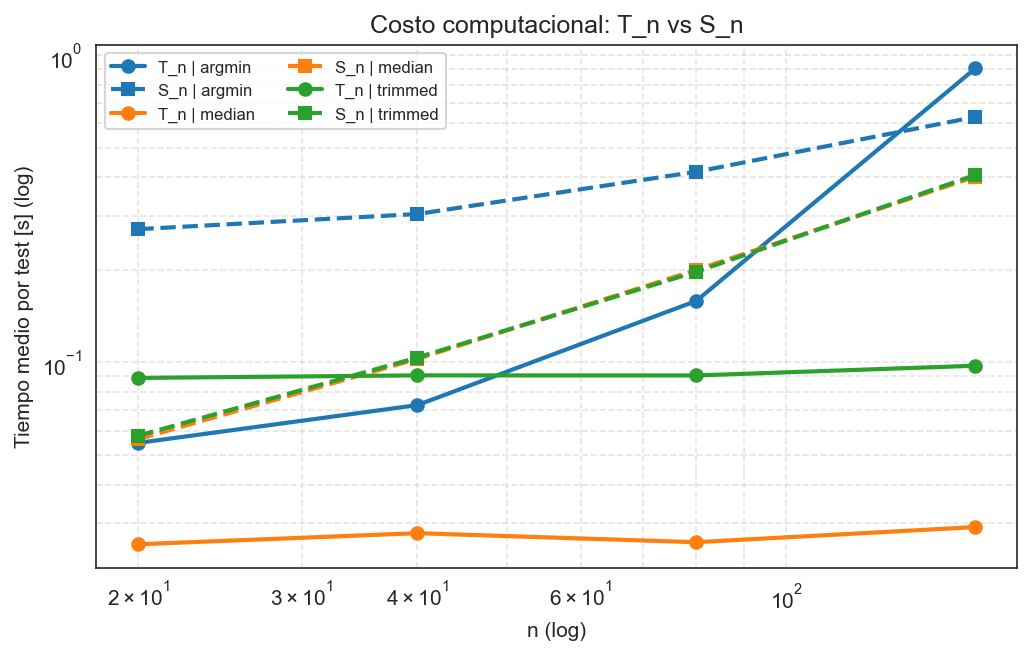
\includegraphics[width=0.85\textwidth]{../results/figures/compare_tn_vs_sn_runtime.png}
  \caption{Comparativa de tiempos $T_n$ vs.\ $S_n$ por estimador y $n$.}
  \label{fig:compare-runtime}
\end{figure}

La Figura~\ref{fig:tradeoff-tn} ilustra el tradeoff potencia--costo en $T_n$: el argmin ofrece potencia inferior a un costo $100\times$ mayor que la mediana bajo Gamma, lo que lo hace la elección menos atractiva para $T_n$. En $S_n$, en cambio, el argmin es competitivo en tiempo y simultáneamente el más potente (ver Figura~\ref{fig:compare-potencia}), gracias a la diferenciabilidad de $S_n$ que permite un optimizador de orden superior.


% =========================================================
\section{Discusión}
\subsection{¿Cómo afectan los distintos $w(t)$ y la elección de $q$ al desempeño de $S_n$?}

En primer lugar, respecto a la elección de \(w(t)\), se observa que las tres alternativas consideradas producen comportamientos similares. Ya que la potencia aumenta conforme crece el tamaño muestral \(n\), alcanzando valores cercanos a 1 en la mayoría de escenarios. Sin embargo, sí aparecen diferencias relevantes en la rapidez con que esto ocurre.

La ponderación Laplace muestra una convergencia más rápida hacia potencia alta, especialmente frente al escenario Pareto. Esto sugiere que asignar mayor peso relativo a regiones alejadas del origen permite capturar mejor desviaciones de simetría asociadas a colas asimétricas. En contraste, los pesos gaussianos tienden a concentrar mayor masa alrededor de \(t=0\), privilegiando información local de baja frecuencia. Esto produce un comportamiento algo más estable, aunque en algunos escenarios requiere tamaños muestrales ligeramente mayores para alcanzar el mismo nivel de potencia.

Entre los pesos gaussianos, la diferencia entre \(\sigma=0.5\) y \(\sigma=1.0\) es moderada. El caso \(\sigma=0.5\) concentra aún más la integral cerca del origen, mientras que \(\sigma=1.0\) distribuye el peso sobre una región más amplia. Empíricamente no se observan diferencias dramáticas entre ambas, aunque \(w=\mathrm{gauss}_{1.0}\) parece ser más estable.

Por otra parte, el parámetro \(q\) controla la forma de penalización de las discrepancias. Cuando \(q=1\), el estadístico agrega desviaciones de manera aproximadamente lineal, resultando menos sensible a diferencias extremas puntuales. Esto genera un comportamiento más robusto y estable frente a variabilidad muestral. Cuando \(q=2\), las discrepancias grandes reciben una penalización cuadrática, aumentando la sensibilidad del test frente a desviaciones pronunciadas respecto a simetría.

En términos prácticos, esto implica que \(q=2\) puede detectar con mayor facilidad asimetrías marcadas, mientras que \(q=1\) tiende a comportarse mejor cuando la asimetría está distribuida de forma más homogénea a lo largo de la distribución. En las simulaciones $q=1$ resulta sistemáticamente superior a $q=2$ con mediana y media afeitada (por ejemplo, con media afeitada y Pareto a $n=40$ la potencia pasa de $38.5\%$ con $q=2$ a $50\%$ con $q=1$). No obstante, este aumento de sensibilidad también puede amplificar el ruido numérico proveniente de la estimación de la función característica empírica, especialmente para valores grandes de \(t\).

Respecto a la elección del estimador del centro $\hat\theta$, los resultados son matizados (véase el Apéndice). Bajo Cauchy, la mediana exhibe el menor RMSE como estimador puntual, mientras que bajo Uniforme el orden se invierte: el argmin tiene el menor RMSE, y la mediana el mayor. En cuanto a la potencia de $S_n$, el argmin es de hecho \emph{el estimador más potente} cuando es compatible con $q$: para Gamma con $q=2$ y $w_1$, alcanza $47.5\%$ en $n=40$ frente al $32\%$ de la mediana; ventaja que se mantiene en todas las distribuciones alternativas. La explicación es que el argmin minimiza $S_n$ sobre la muestra observada, dejando $S_n^{\text{obs}}$ pequeño pero, simultáneamente, las remuestras bootstrap (provenientes de $sF_n(\hat\theta_{\min})$) producen $S_n^*$ comparablemente pequeño, de manera que la calibración relativa es correcta y el test detecta la asimetría con mayor sensibilidad. La limitación práctica del argmin es su exclusión bajo $q=1$ —ya que el integrando $|\cdot|^{1/2}$ no es diferenciable en sus ceros y la búsqueda en grilla resulta prohibitiva en el bootstrap— por lo que en ese caso solo se evalúan mediana y media afeitada.

De forma conjunta, los resultados sugieren que la elección de \(w(t)\) afecta principalmente la sensibilidad del test frente a distintos tipos de asimetría —especialmente en colas— mientras que \(q\) modula la severidad con que dichas discrepancias son penalizadas. Empíricamente, las configuraciones con peso Laplace o gaussiano de escala intermedia, combinadas con el argmin (cuando $q=2$) o con la media afeitada (cuando $q=1$), presentan el mejor compromiso entre potencia y estabilidad numérica.


% =========================================================
\section{Conclusiones}
\input{6 - conclusiones}

% =========================================================
%\section*{Apéndice}
%
\subsection*{Calidad de los estimadores del centro de simetría}

En esta parte se compara el comportamiento de los tres estimadores del centro de simetría considerados en el proyecto: el estimador por minimización \(\hat\theta_{\min}\), la mediana \(\hat\theta_{\mathrm{med}}\) y la media afeitada \(\hat\theta_\alpha\). La comparación se divide en dos escenarios. Bajo \(H_0\), como la distribución sí es simétrica y el centro verdadero es conocido, se evalúa la precisión de cada estimador mediante RMSE, MAE, sesgo y distribución del error. Bajo \(H_a\), en cambio, no existe un centro verdadero de simetría; por tanto, solo se analiza la estabilidad de los estimadores a través de la variabilidad de \(\hat\theta\) entre réplicas.

\subsubsection*{Precisión bajo \texorpdfstring{$H_0$}{H0}: RMSE, MAE y sesgo}

Para evaluar directamente la calidad de los estimadores bajo \(H_0\), se consideran las dos distribuciones simétricas usadas en las simulaciones: Cauchy\((2,1)\) y Uniforme\((1,3)\). En ambos casos el centro verdadero es \(\theta=2\), por lo que se reportan el RMSE, el MAE y el sesgo empírico de cada estimador.


\begin{figure}[H]
  \centering
  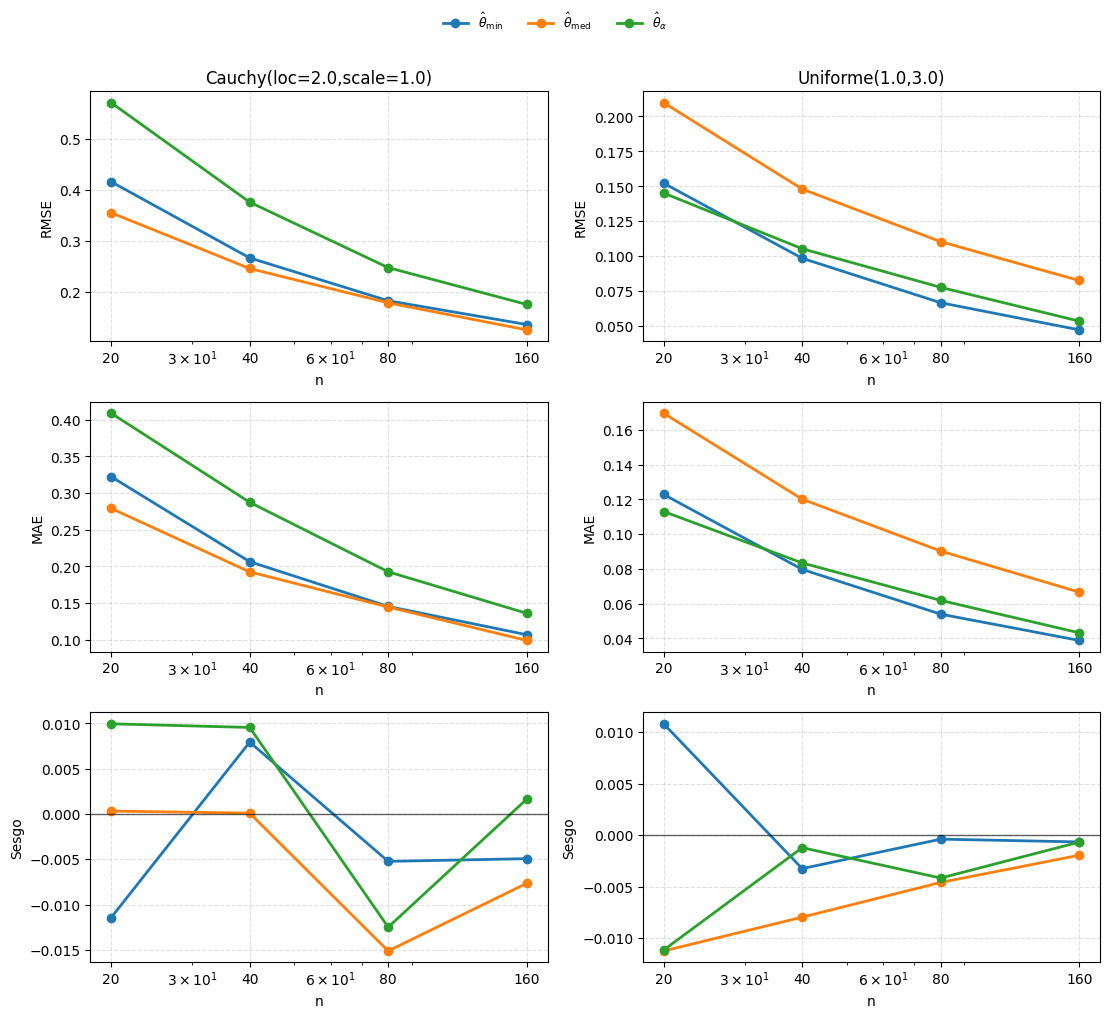
\includegraphics[width=\textwidth]{../results/figures/discusion/theta_estimators_h0_all_metrics.png}
  \caption{Comparación de los estimadores del centro bajo \(H_0\). Se muestran RMSE, MAE y sesgo para Cauchy\((2,1)\) y Uniforme\((1,3)\), usando \(n\in\{20,40,80,160\}\).}
  \label{fig:theta-estimators-h0}
\end{figure}

En la distribución Cauchy, la mediana presenta el mejor comportamiento global en RMSE y MAE para todos los tamaños muestrales. Esto es consistente con la robustez de la mediana frente a colas pesadas. El estimador \(\hat\theta_{\min}\) mejora al aumentar \(n\) y se acerca mucho a la mediana para \(n=80\) y \(n=160\), mientras que la media afeitada muestra errores mayores, especialmente para muestras pequeñas.

En la distribución Uniforme, el patrón cambia: \(\hat\theta_{\min}\) tiene el menor RMSE y MAE para \(n\ge 40\), mientras que la media afeitada es competitiva para \(n=20\). La mediana resulta menos eficiente en este caso, con errores sistemáticamente mayores. Esto sugiere que, en distribuciones simétricas de soporte acotado, el estimador por minimización aprovecha mejor la estructura global de la muestra.

El sesgo empírico es pequeño para los tres estimadores y tiende a cero al crecer \(n\). Por tanto, las diferencias principales entre ellos no se deben a sesgo sistemático, sino a varianza y sensibilidad frente a colas pesadas. En conjunto, \(\hat\theta_{\min}\) es el estimador más competitivo bajo soporte acotado, mientras que la mediana es preferible cuando hay colas pesadas.

\subsubsection*{Distribución de los errores de estimación bajo \texorpdfstring{$H_0$}{H0}}

Para complementar las métricas anteriores, se analiza la distribución completa de los errores \(\hat\theta-\theta\). Esto permite observar no solo el error promedio, sino también la dispersión y la estabilidad de cada estimador.


\begin{figure}[H]
  \centering
  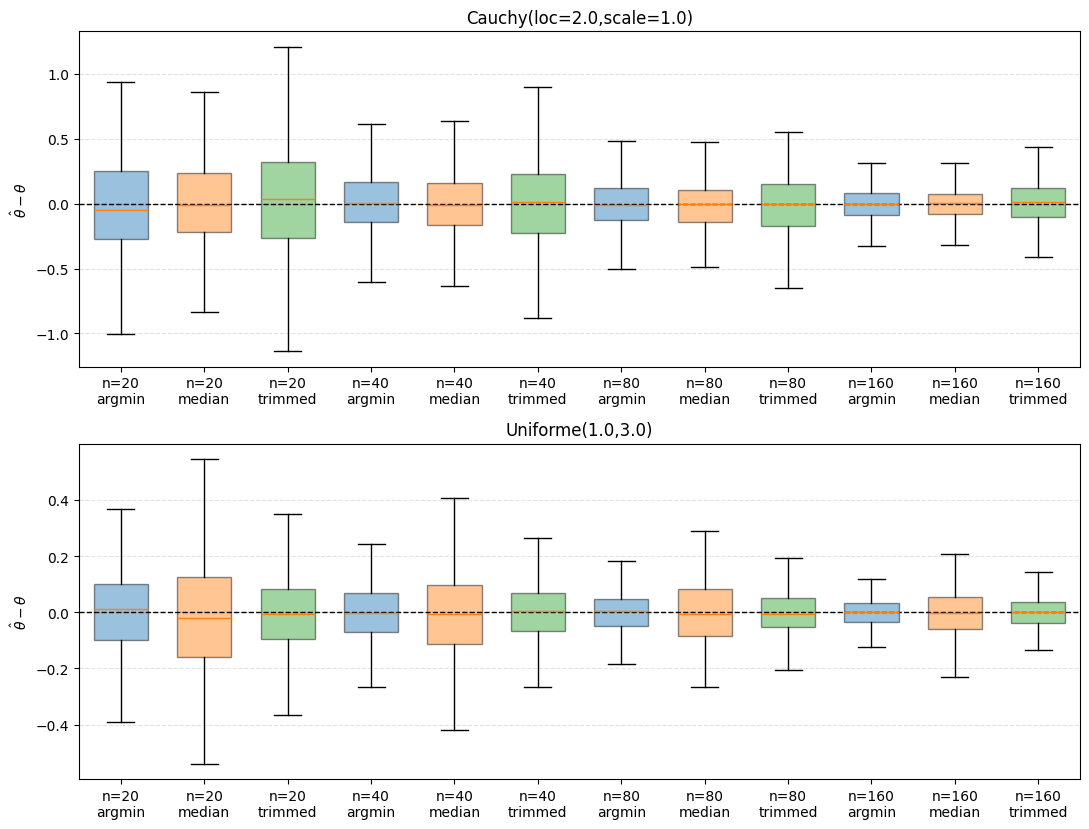
\includegraphics[width=\textwidth]{../results/figures/discusion/theta_estimator_error_boxplots_h0.png}
  \caption{Distribución de los errores de estimación \(\hat\theta-\theta\) bajo \(H_0\), para Cauchy\((2,1)\) y Uniforme\((1,3)\). Se muestran diagramas de caja para \(\hat\theta_{\min}\), la mediana y la media afeitada, en \(n\in\{20,40,80,160\}\).}
  \label{fig:theta-error-boxplots-h0}
\end{figure}

La Figura~\ref{fig:theta-error-boxplots-h0} confirma las conclusiones anteriores. En ambos modelos, la dispersión de \(\hat\theta-\theta\) disminuye al aumentar \(n\), como es esperable por consistencia. Sin embargo, la forma en que se concentra la distribución del error depende del estimador y de la distribución subyacente.

Bajo Cauchy, la mediana presenta cajas más estrechas y centradas alrededor de \(0\) que los otros estimadores, especialmente para \(n=20\) y \(n=40\), lo que refuerza su mayor estabilidad en presencia de colas pesadas. El estimador \(\hat\theta_{\min}\) también mejora con \(n\), pero exhibe una dispersión algo mayor en muestras pequeñas. La media afeitada es la más variable, en concordancia con sus mayores valores de RMSE y MAE.

Bajo Uniforme, en cambio, \(\hat\theta_{\min}\) y la media afeitada muestran una dispersión menor que la mediana para \(n\ge 40\). En particular, \(\hat\theta_{\min}\) exhibe cajas más compactas para \(n=80\) y \(n=160\), lo que explica su ventaja en RMSE y MAE en esta distribución. La mediana conserva un sesgo pequeño, pero su variabilidad es mayor de forma sistemática.

En conjunto, los diagramas de caja muestran que las diferencias entre estimadores provienen principalmente de la variabilidad de \(\hat\theta\), más que de sesgos apreciables. Esto respalda la conclusión de que la mediana es preferible bajo colas pesadas, mientras que \(\hat\theta_{\min}\) resulta más eficiente en distribuciones simétricas de soporte acotado.


\subsubsection*{Estabilidad bajo \texorpdfstring{$H_a$}{Ha}}

Bajo \(H_a\), las distribuciones consideradas no son simétricas; por tanto, no existe un verdadero centro de simetría contra el cual comparar los estimadores. En este caso, no se calculan RMSE ni sesgo respecto a un parámetro real. En su lugar, se analiza la estabilidad de \(\hat\theta\), medida por su desviación estándar entre réplicas de Monte Carlo.


\begin{figure}[H]
  \centering
  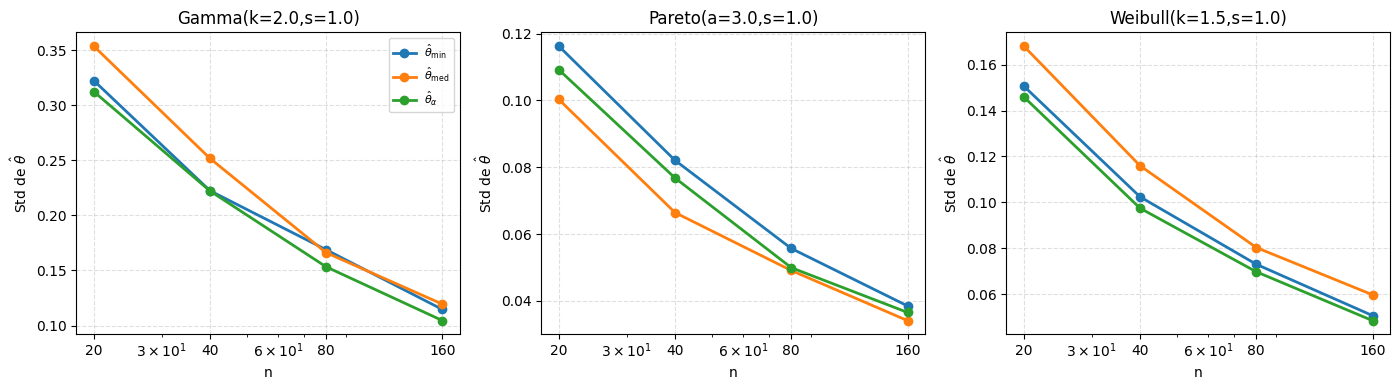
\includegraphics[width=\textwidth]{../results/figures/discusion/theta_estimator_std_ha.png}
  \caption{Desviación estándar de \(\hat\theta\) bajo \(H_a\), para las distribuciones Gamma\((2,1)\), Pareto\((3,1)\) y Weibull\((1.5,1)\).}
  \label{fig:theta-std-ha}
\end{figure}

Bajo \(H_a\) no existe un verdadero centro de simetría, por lo que ya no tiene sentido comparar los estimadores mediante RMSE o sesgo respecto a un parámetro real. En este caso, el interés se desplaza hacia la estabilidad de \(\hat\theta\), medida aquí por su desviación estándar a través de las réplicas de Monte Carlo.

La Figura~\ref{fig:theta-std-ha} muestra que la variabilidad de los tres estimadores disminuye con \(n\) en las tres distribuciones asimétricas consideradas. Sin embargo, el orden relativo entre ellos depende de la forma de la distribución. En Gamma y Weibull, la media afeitada \(\hat\theta_\alpha\) es la más estable en casi todos los tamaños muestrales, seguida muy de cerca por \(\hat\theta_{\min}\), mientras que la mediana presenta mayor dispersión. En cambio, bajo Pareto, la mediana resulta ser el estimador más estable para todos los \(n\), lo cual es coherente con su mayor robustez frente a colas pesadas.

En conjunto, estos resultados sugieren que, fuera de la hipótesis de simetría, la elección del estimador depende en buena medida de la severidad de la asimetría y del peso de las colas. La media afeitada ofrece la mejor estabilidad en alternativas moderadamente asimétricas como Gamma y Weibull, mientras que la mediana vuelve a destacar cuando la asimetría viene acompañada de colas más pesadas, como en Pareto.




Se evalúan los tres estimadores del centro usados en las pruebas bootstrap,
ahora como estimadores puntuales de la localización ($R=500$ réplicas Monte Carlo
por combinación distribución $\times$ $n$):

\begin{enumerate}
  \item $\hat\theta_{\min}$ \textbf{(argmin de $T_n$, Schuster-Narvarte)}: minimizador exacto de $T_n(\theta)$ obtenido por el algoritmo combinatorio de Schuster-Narvarte.
  \item $\hat\theta_{\mathrm{med}}$ \textbf{(mediana muestral)}: minimiza $\sum_i|X_i-\theta|$. Máxima robustez (breakdown $50\%$), asintóticamente eficiente para distribuciones de Cauchy.
  \item $\hat\theta_\alpha$ \textbf{(media afeitada $10\%$)}: media de los datos sin el $10\%$ extremo en cada cola.
\end{enumerate}

% -----------------------------------------------------------
\subsubsection*{Bajo \texorpdfstring{$H_0$}{H0}: sesgo y RMSE}

\begin{figure}[H]
  \centering
  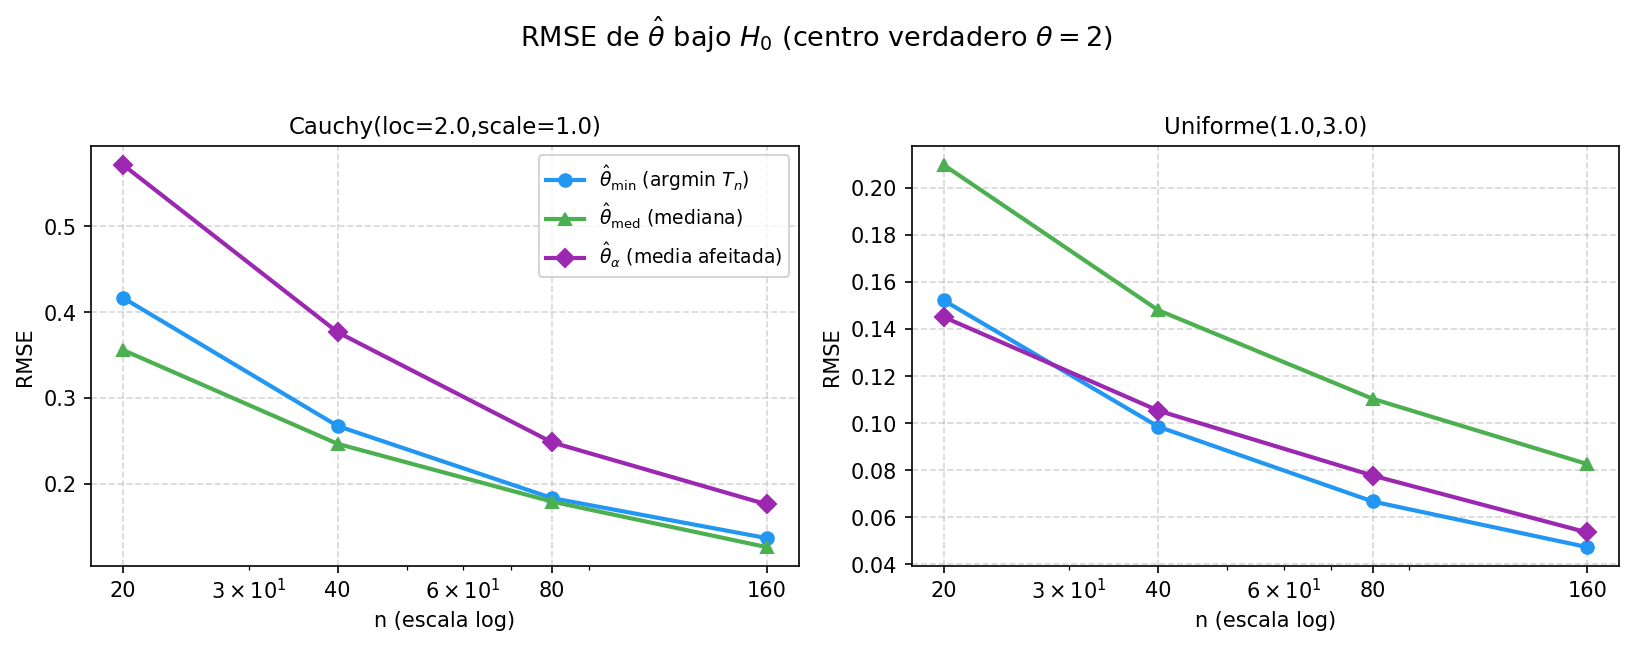
\includegraphics[width=\textwidth]{../results/figures/apendice_rmse_h0.png}
  \caption{
    \textbf{RMSE} de los tres estimadores bajo $H_0$ en función de $n$ (escala log).
    Izquierda: Cauchy$(2,1)$ (colas pesadas); derecha: Uniforme$(1,3)$ (colas ligeras).
    El centro verdadero es $\theta=2$ en ambos casos.
  }
  \label{fig:apendice-rmse-h0}
\end{figure}

Los patrones de RMSE difieren según la distribución nula:

\begin{itemize}
  \item \textbf{Cauchy$(2,1)$} (Figura~\ref{fig:apendice-rmse-h0}, izquierda).
    La mediana es el estimador con menor RMSE en todos los $n$ (es el estimador de máxima verosimilitud de la Cauchy). El argmin ocupa el segundo lugar. La media afeitada presenta el mayor RMSE, pues no es eficiente bajo colas tan pesadas: para $n=20$ su RMSE es $0.572$, frente a $0.356$ de la mediana.

  \item \textbf{Uniforme$(1,3)$} (Figura~\ref{fig:apendice-rmse-h0}, derecha).
    El orden se invierte: la media afeitada y el argmin tienen los menores RMSE (virtualmente iguales para $n\ge40$), mientras que la mediana tiene el \emph{mayor} RMSE. Para $n=160$: argmin~$0.047$, media afeitada~$0.054$, mediana~$0.083$. Esto se explica porque para la Uniforme, cuya densidad es constante, la media de la muestra transporta más información sobre el centro que la observación mediana; la media afeitada captura esto parcialmente, y el argmin la explota completamente al integrar todos los pares de Walsh.
\end{itemize}

\begin{figure}[H]
  \centering
  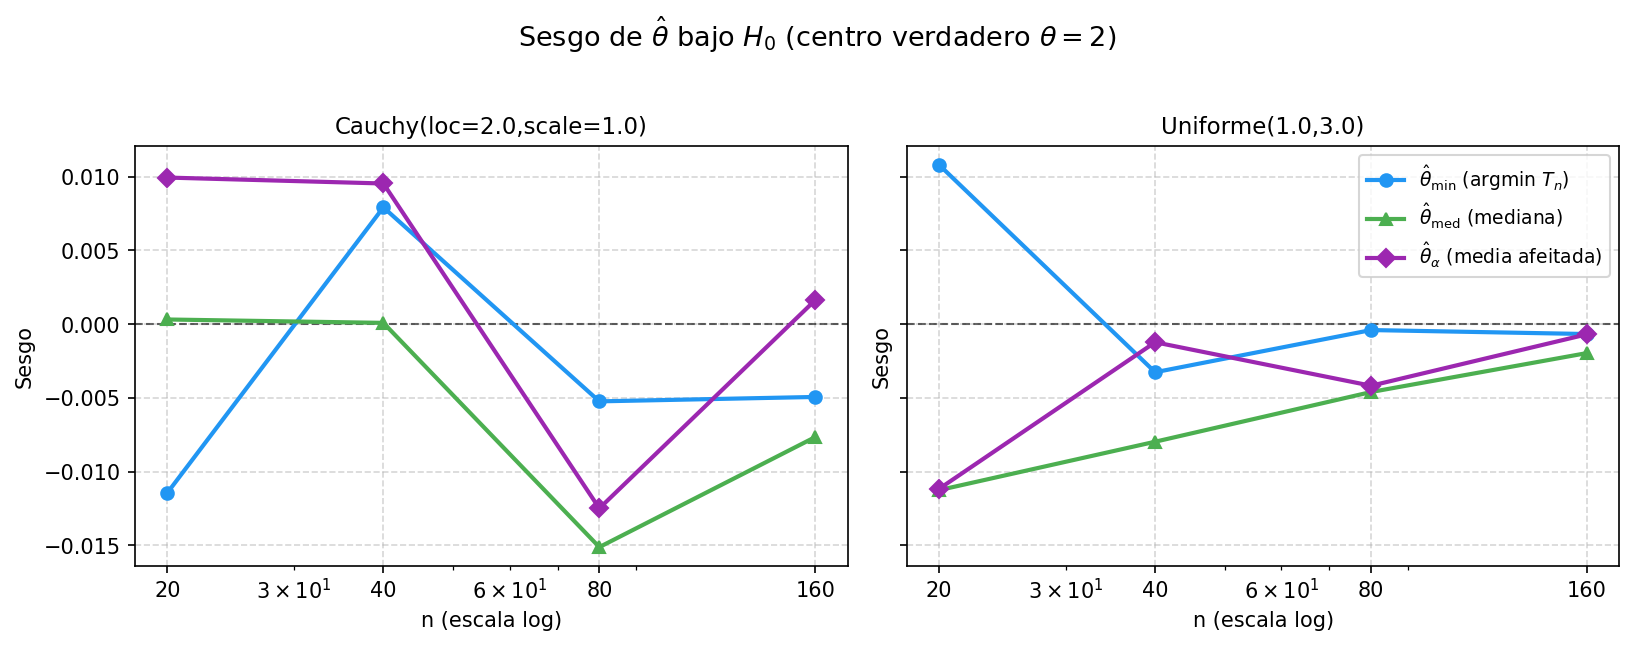
\includegraphics[width=\textwidth]{../results/figures/apendice_bias_h0.png}
  \caption{
    \textbf{Sesgo} de los tres estimadores bajo $H_0$ ($\theta=2$) en función de $n$.
    La línea punteada marca sesgo cero. Las desviaciones respecto a cero son
    estadísticamente indistinguibles de cero ($R=500$, $\mathrm{SE}\approx\mathrm{RMSE}/\sqrt{500}$).
  }
  \label{fig:apendice-bias-h0}
\end{figure}

Como muestra la Figura~\ref{fig:apendice-bias-h0}, los tres estimadores son prácticamente insesgados bajo $H_0$ ($|\text{sesgo}|<0.015$ en todos los casos). Este resultado confirma que el conservatismo del test $T_n$ con estimador argmin no proviene de un sesgo en la estimación de $\theta$, sino de que minimizar $T_n$ sobre los datos observados reduce directamente el estadístico.

\begin{figure}[H]
  \centering
  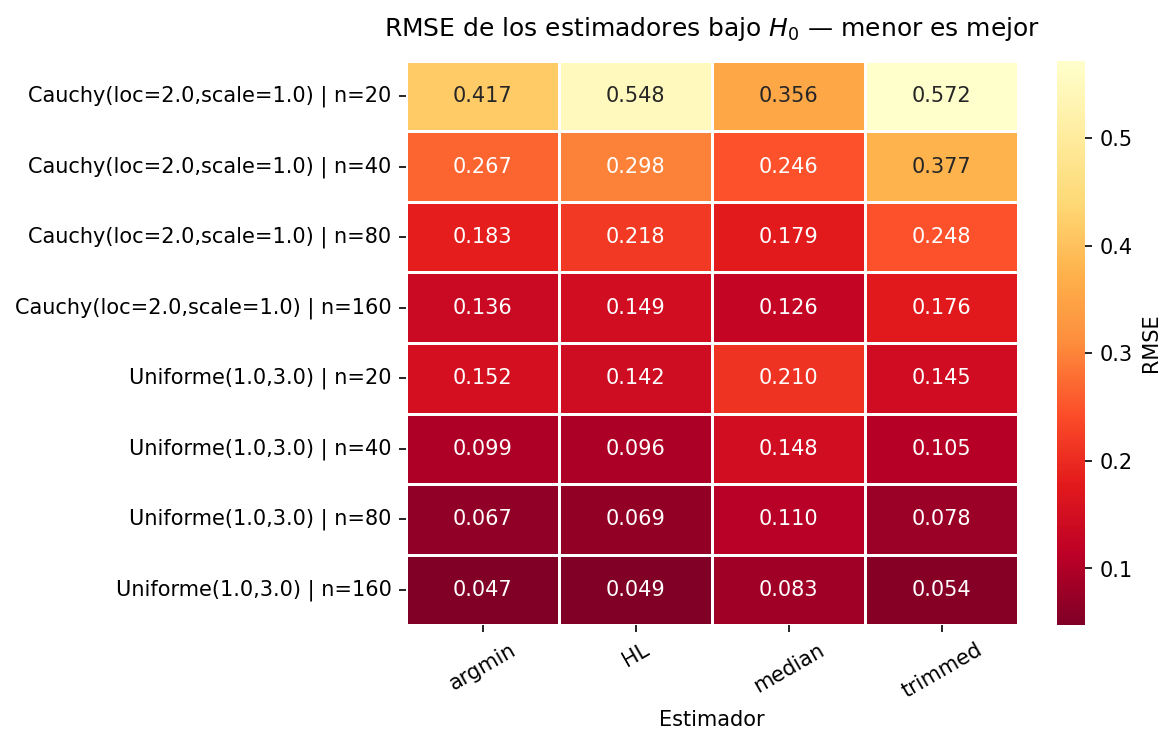
\includegraphics[width=\textwidth]{../results/figures/apendice_rmse_heatmap.png}
  \caption{
    \textbf{Heatmap de RMSE} bajo $H_0$: tonos más claros indican menor RMSE (mejor estimador).
    El argmin domina bajo Uniforme; la mediana domina bajo Cauchy.
  }
  \label{fig:apendice-rmse-heatmap}
\end{figure}

% -----------------------------------------------------------
\subsubsection*{Bajo \texorpdfstring{$H_a$}{Ha}: distribución de \texorpdfstring{$\hat\theta$}{theta hat}}

Bajo las distribuciones alternativas (Gamma, Weibull, Pareto) no existe un centro de simetría verdadero; se estudia dónde ``localiza'' cada estimador.

\begin{figure}[H]
  \centering
  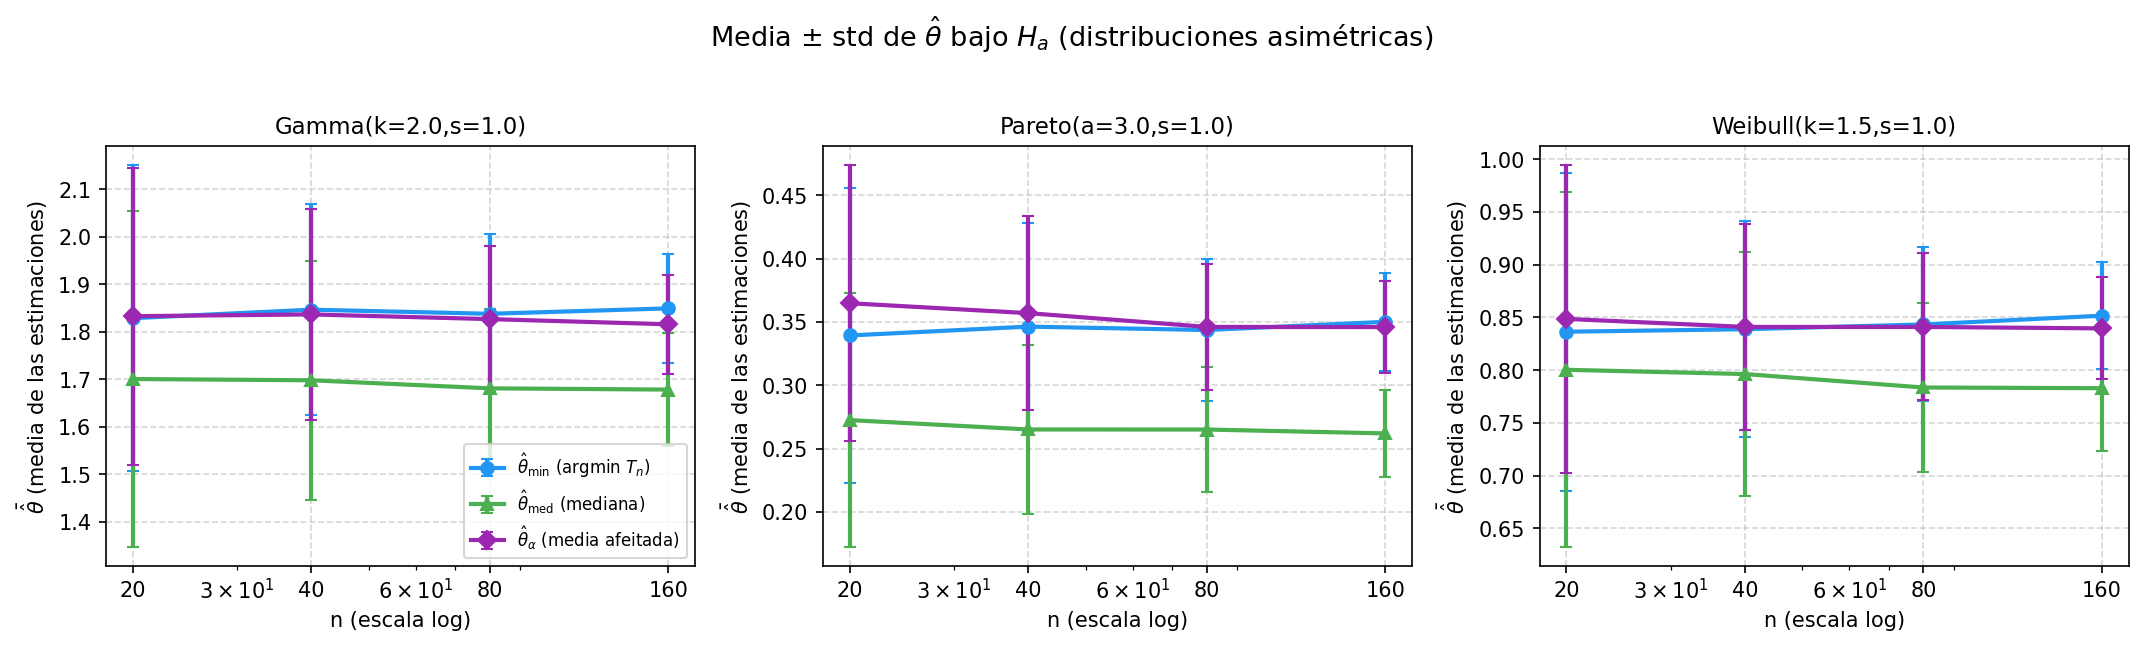
\includegraphics[width=\textwidth]{../results/figures/apendice_theta_ha.png}
  \caption{
    \textbf{Media $\pm$ desviación estándar} de $\hat\theta$ bajo $H_a$:
    Gamma$(2,1)$ (izquierda), Weibull$(1.5,1)$ (centro) y Pareto$(3,1)$ (derecha).
    La distribución de $\hat\theta$ converge con $n$ hacia un valor determinístico
    específico de cada estimador.
  }
  \label{fig:apendice-theta-ha}
\end{figure}

Las diferencias entre estimadores son más pronunciadas bajo $H_a$:

\begin{itemize}
  \item \textbf{Mediana ($\hat\theta_{\mathrm{med}}$)}: converge al cuantil $0.5$ de la distribución asimétrica.
    Para Gamma$(2,1)$: $\bar{\hat\theta}\approx 1.68$ (cuantil $0.5$ teórico $\approx 1.68$); para Pareto$(3,1)$: $\bar{\hat\theta}\approx 0.26$.

  \item \textbf{Argmin ($\hat\theta_{\min}$)}: localiza el centro en un punto intermedio entre la mediana y la media de la distribución. Para Gamma$(2,1)$: $\bar{\hat\theta}\approx 1.84$; para Pareto$(3,1)$: $\bar{\hat\theta}\approx 0.35$. Este desplazamiento positivo respecto a la mediana es propio de un estimador que promedia pares (Walsh averages): bajo asimetría derecha, hay más pares con suma elevada que baja, desplazando el argmin hacia arriba.

  \item \textbf{Media afeitada}: perfil muy similar al argmin ($\bar{\hat\theta}\approx 1.82$--$1.84$ para Gamma), con ligera ventaja en varianza para $n$ grande.

  \item \textbf{Variabilidad}: la desviación estándar decrece como $\mathcal{O}(n^{-1/2})$ en los tres estimadores; no hay diferencias apreciables de dispersión entre ellos para $n\ge 40$.
\end{itemize}

La diferencia en la localización de $\hat\theta$ entre la mediana y los demás estimadores es relevante para la potencia del test: el argmin ubica el centro en un punto que hace la distribución empírica ``más alejada'' de su simetrización, de modo que $T_n(\hat\theta_{\min})$ resulta comparativamente mayor bajo $H_a$ que $T_n(\hat\theta_{\mathrm{med}})$. El bootstrap calibra este efecto correctamente (también minimiza sobre cada remuestra), y el resultado neto es la mayor potencia del argmin observada en la Sección~\ref{sec:potencia}.

\newpage
\bibliography{ref}
\bibliographystyle{plain}

\newpage
\section*{Checklist del Proyecto 2: Estadística No Paramétrica}

\noindent\textcolor{green}{$\blacksquare$} Gabriel \quad
\textcolor{red}{$\blacksquare$} Ing.\ Juan David \quad
\textcolor{blue}{$\blacksquare$} Luis Tejón \quad
\textcolor{orange}{$\blacksquare$} Claudio (IA) \quad
\textcolor{purple}{$\blacksquare$} Todos

\subsection*{Fase 1: Estructura y Configuración del Repositorio}
\begin{itemize}
    \item[\textbf{[\checkmark]}] \textcolor{blue}{(Luis Tejón)} Migrar plantilla LaTeX del Proyecto 1 y limpiar contenido obsoleto.
    \item[\textbf{[\checkmark]}] \textcolor{blue}{(Luis Tejón)} Configurar repositorio GitHub y sincronización Overleaf vía git.
    \item[\textbf{[\checkmark]}] \textcolor{blue}{(Luis Tejón)} Crear y configurar archivo \texttt{.gitignore} en la raíz.
    \item[\textbf{[ ]}] \textcolor{blue}{(Luis Tejón)} Separar la lógica de ejecución en Jupyter Notebooks (\texttt{0\_generar\_muestras}, \texttt{1\_procesar\_estadisticos}, \texttt{2\_graficos}).
    \item[\textbf{[ ]}] \textcolor{purple}{(Todos)} Revisar que la estructura modular del código de Claudio sea clara y navegable.
\end{itemize}

\subsection*{Fase 2: Implementación Matemática}
\begin{itemize}
    \item[\textbf{[ ]}] \textcolor{orange}{(Claudio)} \textbf{Hacer TODO el código.}
    \item[\textbf{[ ]}] \textcolor{orange}{(Claudio)} Documentar cada función con descripción, parámetros, retorno y ejemplo de uso.
    \item[\textbf{[ ]}] \textcolor{green}{(Gabriel)} Revisar que la simetrización $sF_n(\theta)$ y el estadístico $T_n$ estén correctamente implementados; contrastar con cálculo manual en muestra pequeña simétrica.
    \item[\textbf{[ ]}] \textcolor{red}{(Ing. Juan David)} Revisar que $c_n(t)$ y el estadístico $S_n$ estén correctos para $q=1$ y $q=2$; verificar que $c_s(t)=\|c_n(t)\|$.
    \item[\textbf{[ ]}] \textcolor{blue}{(Luis Tejón)} Revisar los tres estimadores del centro de simetría (argmin, mediana, media afeitada) para ambos tests.
    \item[\textbf{[ ]}] \textcolor{green}{(Gabriel)} Revisar el procedimiento bootstrap de $T_n$: verificar que las remuestras se generan de $sF_n(\tilde\theta)$ y que el p-valor se calcula correctamente.
    \item[\textbf{[ ]}] \textcolor{red}{(Ing. Juan David)} Revisar el procedimiento bootstrap de $S_n$ y las funciones de peso $w(t)$ candidatas.
    \item[\textbf{[\checkmark]}] \textcolor{blue}{(Luis Tejón)} Agregar y revisar la medición de tiempo de ejecución por test, estimador y configuración.
\end{itemize}

\subsection*{Fase 3: Diseño y Ejecución de Simulaciones}
\begin{itemize}
    \item[\textbf{[\checkmark]}] \textcolor{red}{(Ing. Juan David)} Definir parámetros de las distribuciones bajo $H_0$ (Uniforme no centrada, Cauchy con localización $\neq 0$) y verificar generadores.
    \item[\textbf{[\checkmark]}] \textcolor{green}{(Gabriel)} Definir parámetros de las distribuciones bajo $H_a$ (Gamma, Weibull, Pareto) y verificar generadores.
    \item[\textbf{[ ]}] \textcolor{green}{(Gabriel)} Realizar estudio piloto para fijar los tamaños muestrales $n$ adecuados.
    \item[\textbf{[ ]}] \textcolor{red}{(Ing. Juan David)} Diseñar la matriz experimental completa: 2 tests $\times$ 3 estimadores $\times$ $w(t)$ candidatas $\times$ $q\in\{1,2\}$ $\times$ distribuciones $\times$ tamaños $n$.
    \item[\textbf{[ ]}] (Cualquiera) Ejecutar simulaciones definitivas con $B=500$ y $R$ réplicas Monte Carlo acordadas.
    \item[\textbf{[\checkmark]}] \textcolor{blue}{(Luis Tejón)} Almacenar resultados de potencia, error Tipo I y tiempos en formato reproducible (CSV/Parquet).
\end{itemize}

\subsection*{Fase 4: Visualización y Gráficos}
\begin{itemize}
    \item[\textbf{[\checkmark]}] \textcolor{blue}{(Luis Tejón)} Gráfico de tasa de Error Tipo I bajo $H_0$ con banda de fluctuación $\sigma_{\hat\alpha}$.
    \item[\textbf{[ ]}] \textcolor{red}{(Ing. Juan David)} Heatmap de potencia empírica por test, estimador de $\theta$ y distribución alternativa.
    \item[\textbf{[ ]}] \textcolor{green}{(Gabriel)} Comparativa de potencia para distintas $w(t)$ y para $q=1$ vs.\ $q=2$ en $S_n$.
    \item[\textbf{[\checkmark]}] \textcolor{blue}{(Luis Tejón)} Gráfico de tiempos de ejecución y scatter de Costo Computacional vs.\ Potencia.
    \item[\textbf{[ ]}] \textcolor{red}{(Ing. Juan David)} Densidades teóricas de las distribuciones empleadas (ilustrativo).
\end{itemize}

\subsection*{Fase 5: Redacción del Informe}
\begin{itemize}
    \item[\textbf{[\checkmark]}] \textcolor{green}{(Gabriel)} Introducción (sección 0): problema de simetría univariada y motivación del enfoque bootstrap.
    \item[\textbf{[\checkmark]}] \textcolor{red}{(Ing. Juan David)} Marco Teórico: definición de simetría, simetrización empírica $sF_n(\theta)$ y motivación del estadístico $T_n$.
    \item[\textbf{[\checkmark]}] \textcolor{blue}{(Luis Tejón)} Marco Teórico: función característica empírica $c_n(t)$ y propiedad clave ($c(t)\in\mathbb{R}\iff X$ simétrica en $0$).
    \item[\textbf{[\checkmark]}] \textcolor{green}{(Gabriel)} Marco Teórico: definición de $S_n$, justificación de $c_s(t)=\|c_n(t)\|$ y rol de $w(t)$ y $q$.
    \item[\textbf{[ ]}] \textcolor{red}{(Ing. Juan David)} Enunciar el resultado teórico de Arcones \& Giné que justifica la validez del bootstrap (sin demostración).
    \item[\textbf{[\checkmark]}] \textcolor{green}{(Gabriel)} Discusión teórica: demostrar que $X\sim\text{sim}(\theta)\iff c(t)=e^{it\theta}c_0(t)$ con $c_0$ real.
    \item[\textbf{[ ]}] \textcolor{blue}{(Luis Tejón)} Metodología (sección 2): protocolo Monte Carlo, diseño experimental y estimadores del centro de simetría.
    \item[\textbf{[ ]}] \textcolor{red}{(Ing. Juan David)} Implementación (sección 3): descripción del código con fragmentos clave, apoyándose en la documentación de Claudio.
    \item[\textbf{[ ]}] \textcolor{green}{(Gabriel)} Resultados: control del Error Tipo I y cumplimiento del nivel bajo $H_0$.
    \item[\textbf{[ ]}] \textcolor{blue}{(Luis Tejón)} Resultados: potencia empírica bajo $H_a$ y comparativa $T_n$ vs.\ $S_n$.
    \item[\textbf{[ ]}] \textcolor{red}{(Ing. Juan David)} Resultados: tiempos de ejecución y análisis de complejidad computacional.
    \item[\textbf{[ ]}] \textcolor{blue}{(Luis Tejón)} Discusión: ¿qué estimador del centro funciona mejor? ¿qué test es preferible y en qué escenarios?
    \item[\textbf{[ ]}] \textcolor{green}{(Gabriel)} Discusión: ¿cómo afectan las distintas $w(t)$ y la elección de $q$ al desempeño de $S_n$?
    \item[\textbf{[ ]}] \textcolor{red}{(Ing. Juan David)} Discusión: tradeoff entre costo computacional y potencia.
    \item[\textbf{[ ]}] \textcolor{purple}{(Todos)} Conclusiones (sección 6): ¿cuál de los dos tests es preferible considerando potencia, nivel y costo?
    \item[\textbf{[ ]}] \textcolor{purple}{(Todos)} Revisión final del documento (ortografía, coherencia notacional, citas).
    \item[\textbf{[ ]}] (Cualquiera) Subir el informe y código a Bloque Neón antes del \textbf{miércoles 27 de mayo de 2026 a las 11:00 pm}.
\end{itemize}

\end{document}